\chapter{Introduction au Big Data} \label{chap:big-data-intro}
	
	\section{Introduction}
		Big Data est un terme associé aux données massives, rapidement générées, ayant une grande diversité où les  outils traditionnels sont incapables de gérer ces données. La complexité du Big Data est dû au  fait que tout type de données peut être utilisé, et ce en vue de livrer la bonne information à la bonne personne et au bon moment dans le but d'aider à prendre les bonnes décisions. Dans ce chapitre, nous  présentons brièvement un des processus d'analyse de données. Ensuite, nous décrivons quelques concepts impliqués dans un processus d'analyse des données massives. Enfin, nous parcourons un ensemble de technologies utilisées dans l'analyse des données à grande échelle.
			
	\section{Processus d'analyse de données massives}
	%668
	
Les étapes d'un processus d'analyse de données, à grande échelle ou non, sont différentes selon le processus adopté.  Ce dernier peut impliquer plusieurs besoins et concepts. En particulier, on note le besoin au stockage de données massives, au traitement de données massives et le besoin à la visualisation des résultats des traitements appliqués. Le choix du traitement à appliquer sur les données est dirigé par les objectifs de  l'analyse menée. Par exemple, une analyse peut envisager la création d'un système de recommandations dans les sites Internet, la conception d'un outil de prédiction basé sur les données historiées, un système de suivi en temps réel, etc.  Ces applications appuient sur des algorithmes basés sur les mathématiques, en particulier les mathématiques statistiques et probabilistes. Afin d'assurer l'efficacité de l'analyse de données massives, la coopération de plusieurs ressources accélère considérablement les étapes de l'analyse, c'est ce que l'informatique distribuée a apporté.


\paragraph{Exemple d'un  processus d'analyse de données} \label{sec:process-data-analysis}~

Le processus d'analyse de données passe généralement par des étapes classiques. A ces étapes peuvent s'ajouter d'autres étapes intermédiaires ou supplémentaires. 
Pour précision, non seulement  ces étapes peuvent s'appliquer dans le cas  où les données sont volumineuses,  mais aussi dans le cas des données manipulées par des outils traditionnels comme les bases de données relationnelles. IBM Knowledge Center \footnote{Source : \url{https://www.ibm.com/support/knowledgecenter/fr/SSEPGG_9.5.0/com.ibm.im.easy.doc/c_dm_process.html}, consultée le $06/08/2018$.} a résumé le processus de l'analyse de données dans les étapes suivantes :
définition de problème, exploration de données, préparation de données, modélisation, évaluation et enfin l'étape de déploiement.


\textbf{Définition de problème} C'est le point d'entrée vers tout projet d'analyse de données. Les objectifs doivent être clairs. A la fin de cette étape, on connait les objectifs de l'analyse, mais pas forcément comment cette analyse va être menée en terme de technologies utilisées,  les méthodes statistiques, etc. \par

\textbf{Exploration de données } Ce que caractérise cette étape, c'est la découverte de la nature  des données, les sources des données, la qualité des données, etc. \par

\textbf{Préparation de données} \label{par:step-preparedata} C'est durant cette phase que se passent les opérations d'ETL (Extract-transform-load), ce sont les opérations de chargement,  nettoyage et de la transformation des données. Durant cette étape aussi que  des tentatives sont faites pour créer le schéma de données.  Dans certains cas, cela amène  à chercher des sources complémentaires de données ou bien de nouvelles transformations à appliquer sur les données. Tel qu'un  schéma comporte les différentes tables, les attributs pertinents et autres. \par

\textbf{Modélisation} A l'issue de cette phase, un modèle de qualité est créé. Un modèle qui doit  répondre aux objectifs précédemment établis. Cette étape implique des principes en statistiques, probabilités, \textit{machine learning}, etc. \par

\textbf{Evaluation} C'est à cette étape qu'on valide le modèle créé à l'étape de  Modélisation. L'évaluation et la validation du modèle prend en compte les objectifs prédéfinis; si le modèle répond aux attentes précédemment exprimées. \par

\textbf{Déploiement}  C'est l'utilisation  des outils existants ou  la mise place d'une solution qui convient aux  besoins spécifiques en terme de visualisation des résultats de l'analyse. \par




	\section{Quelques concepts associés au Big Data}

Etant donné que le domaine du Big Data implique plusieurs concepts, nous présentons une liste de concepts  non exhaustive. 

		\subsection{Définition du Big Data : Volume, Vélocité, Variété et Véracité}
		
		IBM définit le Big Data suivant les quatre dimensions suivants : volume, variété, vélocité et véracité. 
		\paragraph{Volume de données}~
		La quantité de données manipulées par les outils traditionnels de la gestion des données est de l'ordre de Gigaoctets (GB) et de Téraoctets (TB). Toutefois, le Big Data est mesuré en Pétaoctets (PB), Exaoctets (EB), voire plus. Une des premières applications du Big Data est la recherche dans Word-Wide Web (WWW). Selon une étude (\cite{6567202}, $2013$) de l'International Data Corporation (IDC), le volume de données  va atteindre $40$ Zettaoctets\footnote{ $ 1$ ZB = $1000000000000$ GB } par  entreprise en $2020$ .
		
		\paragraph{Vélocité de données} ~
		le Big Data est généré par des milliards
		d'appareils, les données générées sont communiquées avec la vitesse de la lumière via l'Internet. L'augmentation de la vitesse de l'Internet est une  des raisons ayant contribué à l'augmentation de la vitesse de la génération de données.	
		%la vitesse décrit la fréquence de la génération et du partage des données. Autrement dit, les données sont générées rapidement et doivent être traitées rapidement pour extraire les informations  pertinentes.
		Par exemple, Wallmart (international discount retail chain) génère environ   $2.5$ Pétaoctets de données chaque  heure via les transactions de ses consommateurs\footnote{Source : \url{https://www.bernardmarr.com/default.asp?contentID=690}, consultée le $ 30/06/2018 $.}.
		
		
		
		
		
		\paragraph{Variété de données} \label{variete-data}
		
		Le Big Data inclut toutes les formes des données, des fonctions diversifiés des données et des sources variées des données.
		
		Le premier aspect de la variété  des données massives est la \textbf{forme} de celles-ci. Les données manipulées incluent du texte, des graphes, des cartes, des vidéos, des photos, etc.
		
		Le deuxième aspect de la variété des données massives concerne les \textbf{fonctions} assurées par ces données. Des données sont issues des conversations humaines, d'autres des transactions des consommateurs, ou bien des données archivées, etc.
		
		Les \textbf{sources} du Big Data est le troisième aspect de  variété. Des données sont en provenance des téléphones mobiles, des tablettes ou des ordinateurs portables, des fichiers journaux, du réseau de capteurs, etc. Les sources du Big Data peuvent être classées en trois grandes catégories : communications \textbf{\textit{human to human}} comme les conversations échangées dans les réseaux sociaux, communications \textbf{\textit{ human to machine}} comme l'accès des utilisateurs aux données dans le web et enfin communications \textbf{\textit{machine to machine}} comme les données issues de la communication entre les capteurs dans un réseau de capteurs.
		%au-delà des données des transactions habituelles des consommateurs, les données manipulées sont en provenance de sources différentes et de formats différents. Par exemple: des vidéos, des documents, des commentaires, des données géospatiales, des journaux, etc. Les grands ensembles de données sont constitués de données structurées et non structurées, publiques ou privées, locales ou distantes, partagées ou confidentielles, complètes ou incomplètes, etc.
		
		
		
		\paragraph{Véracité de données}
		
		La véracité concerne la crédibilité et la qualité de données. La mauvaise qualité de données est due à de nombreuses raisons, telles que les pannes techniques comme le dysfonctionnement des appareils comme les capteurs, les erreurs humaines,  etc. De plus, les données peuvent être intentionnellement erronées pour des raisons de concurrence ou des raisons stratégiques.
	
		\subsection{L'architecture standard du Big Data}
		
		L'architecture standard du Big Data présentée dans ce qui suit est celle proposée dans  \cite{anil-big-data}. Cette architecture  est composée des couches suivantes :  \textit{Data sources}, \textit{Data Ingest}, \textit{Batch processing}, \textit{Stream Processing}, \textit{Data organizing}, \textit{Infrastructure}, \textit{Distributed File System} et enfin la couche \textit{Data consuption}. 
		%Pour  chaque couche, il existe au moins une technologie.
		 La Figure \ref{fig:bigdata-architecture} reprend l'organisation des différentes couches de cette architecture.
		 		\begin{figure}[h]
		 	\captionsetup{justification = centering}
		 	\centering
		 	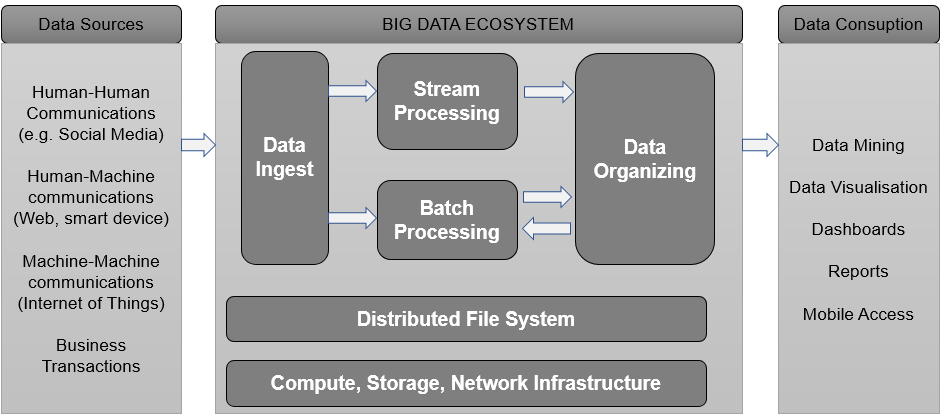
\includegraphics[width=1\linewidth]{illustrations/bigdata-architecture}
		 	\caption{Architecture standard du Big Data \cite{anil-big-data}}
		 	\label{fig:bigdata-architecture}
		 	
		 \end{figure}
		
		Dans un premier temps, les données sont   accueillies   via la couche  \textit{ingest system} par diverses sources de données. Ensuite, les données sont traitées dans deux modes différents:  \textit{stream processing } et  \textit{batch processing}.  Les résultats de ce traitement peuvent être envoyées vers les bases de données NoSQL (\ref{sec:nosql}) pour une utilisation ultérieure, ou bien  utiliser ces résultats comme entrées pour d'autres applications.  Une solution Big Data comprend typiquement  ces  couches logiques. Chaque  couche peut être représentée par une ou plusieurs technologies disponibles. Reprenons chaque couche logique:
		
		
		\begin{description}
			\item[Data sources layer] Le choix des sources de donnés pour une application donnée dépend des objectifs qui dirigent l'analyse en question. Les sources avec leurs différents aspects sont détaillées dans la section \ref{variete-data}.
		
			
		\item[Data Ingest layer] Cette couche permet de récupérer les données depuis les différentes sources de données. Les données sont accueillies à travers des points d'entrées multiples. Ces points  sont capables de recevoir  ces données ayant une vélocité variable ainsi qu'une quantité aussi variable.  Après avoir traversé  la couche \textit{Data Ingest}, les données sont envoyées au \textit{batch processing system}, au \textit{realtime processing system}, ou bien à un système de stockage particulier.
		
		\item[Batch processing layer] Les données reçues sur cette couche sont celles en provenance du \textit{Data Ingest} ou bien d'une des bases de données NoSQL. Ces données sont ensuite traitées, par exemple, en utilisant les techniques de la programmation parallèle en vue de fournir les résultats souhaités dans un temps raisonnable. La présente couche doit avoir connaissance des sources de données, les types de données, les algorithmes qui vont travailler sur ces données et enfin les résultats souhaités. Les résultats des traitements peuvent être utilisés par une des applications ou bien sauvegarder ces données dans une des bases de données adaptées.
		
		
		\item[Stream Processing layer] Cette couche approvisionne les données directement d'une des entrées du \textit{Data Ingest layer}; c'est ce que différencie cette couche de la couche Batch processing layer. En revanche, \textit{Stream Processing} est similaire à la couche   \textit{Batch processing} en matière  des techniques de la programmation parallèle utilisées ainsi que la nécessité d'avoir les détails sur les sources des données, les types de données et les résultats souhaités.
		
		
		\item[Data organizing layer] Le rôle de cette couche est d'organiser les données afin de faciliter l'accès à ces dernières. Ce sont les  données obtenues  de la part de la  couche  \textit{Stream Processing} ainsi que la couche \textit{Batch processing}. Cette couche est représentée par les bases de données NoSQL. 
		
		\item[Infrastructure layer] Cette composante est responsable de la gestion des ressources de stockage, les ressources du calcul et la gestion de la communication. 
		Par exemple, les fonctionnalités de cette couche sont fournies à travers le cloud computing.
		
		\item[Distributed File System layer] Cette couche permet de stocker une grande quantité de données, de sorte que ces données soient rapidement et facilement accessibles à toute les couches qui forment un système du Big Data. C'est ce que assure, par exemple, Hadoop Distributed File System (HDFS).
		
		\item[Data consumption layer] Cette dernière couche utilise les résultats obtenus par les couches de l'analyse. Les résultats fournis peuvent être exprimés avec des rapports, des dashboards, des visualisations, un moteur de recommandation ou tout autre format.
		
	\end{description}
	


	
	\subsection{Les bases de données NoSQL (Not Only SQL) } \label{sec:nosql}
	
	
	\paragraph{Introduction } ~
	
    Au cours de ces dernières années, on constate une révolution dans le stockage de données non structurées ayant une taille importante.  De plus,  les objets à sauvegarder sont complexes; ils sont issus de sources hétérogènes.  Cette complexité a mis en question les performances des bases de données relationnelles. 
	
	Le terme NoSQL est apparu pour la première fois en $ 1998 $. Carlo Strozzi  a parlé des bases de données relationnelles qui n'utilisent pas le SQL comme langage d'interrogation des tables. Des années plus tard, des solutions  open source basées sur ce concept ont vu le jour. 
	
	Les bases de données relationnelles sont conçues pour gérer les données structurées, optimisées pour offrir la précision et la cohérence de données. De plus, elles sont utilisées par la majorité des entreprises pour plusieurs raisons comme   la facilité d'utilisation, la disponibilité de plusieurs produits et développeurs, etc. Ces dernières années, avec l'augmentation exponentielle de la quantité de données générées par certaines entreprises, ces dernières ont constaté l'insuffisance des Systèmes de Gestion de Bases de Données Relationnelles (SGBDR) pour répondre à leurs besoins.
	
    %	\paragraph{ Les besoins auxquels répondent NoSQL}  ~
	
	Les bases de données NoSQL sont conçues pour gérer des  volumes de données importants. Le flux ainsi que la structure de  ces données sont imprévisibles. C'est pourquoi les bases de données relationnelles ne sont pas convenables. L'idée  de des bases de données NoSQL, c'est d'abord assurer la capacité de stocker des données à grande échelle dont leur  quantité  évolue rapidement, voire exponentiellement.  En deuxième lieu, les données stockées  doivent être interrogées  avec efficacité. Les données stockées dans  les bases de données NoSQL n'obéissent pas à un modèle prédéfini comme le cas des bases de données relationnelles. Cette flexibilité est une des caractéristiques des bases de données NoSQL.
	
	
	\paragraph{Types de base de données NoSQL} \label{sec:nosql-database}  ~
	
	Il existe quatre catégories distinctes de bases de données NoSQL. Chaque catégorie répond  à des besoins particuliers. Notamment, on distingue les bases de données clé-valeur, document, graphe et colonne.
	
	
	\subparagraph {Clé-valeur} Une base de données de type clé-valeur repose sur le paradigme clé-valeur; chaque donnée, que ce soit un nombre, du texte ou tout autre type est associé à une clé unique. Cette clé est le seul moyen d'accéder aux données stockées.
	Dans les bases de données NoSQL de type clé-valeur, les enregistrements  n'adhèrent pas à une structure prédéfinie. Par exemple, on peut avoir le premier enregistrement de type entier et le deuxième enregistrement de type texte. Cela assure une forte évolutivité grâce à l'absence d'une structure ou de typage. La Figure \ref{fig:key-value-nosql} reprend un exemple d'une base de données NoSQL de type clé-valeur.

	
	\begin{figure}[H]
		\captionsetup{justification=centering}
		\centering
		\resizebox{.4\textwidth}{!}{
			% Graphic for TeX using PGF
% Title: /home/hayat/report_memoire/illustrations/key-value-nosql.dia
% Creator: Dia v0.97+git
% CreationDate: Sun Dec  2 15:37:59 2018
% For: hayat
% \usepackage{tikz}
% The following commands are not supported in PSTricks at present
% We define them conditionally, so when they are implemented,
% this pgf file will use them.
\ifx\du\undefined
  \newlength{\du}
\fi
\setlength{\du}{15\unitlength}
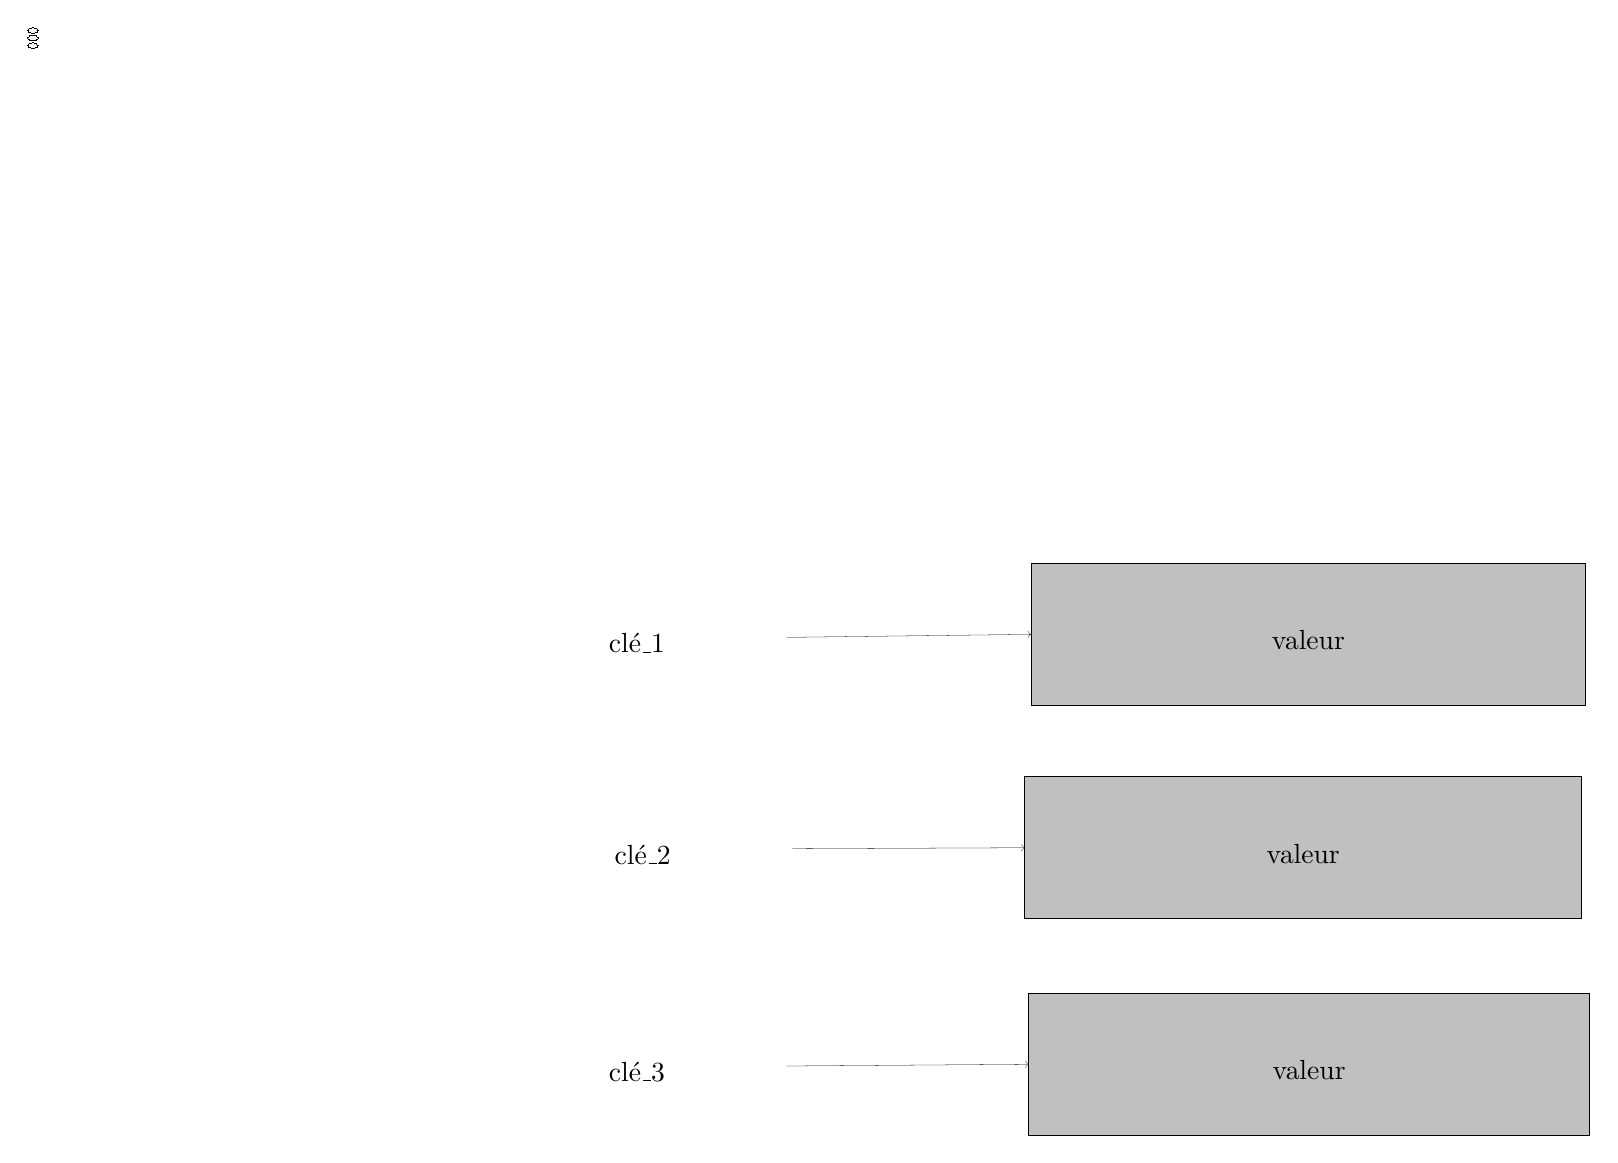
\begin{tikzpicture}[even odd rule]
\pgftransformxscale{1.000000}
\pgftransformyscale{-1.000000}
\definecolor{dialinecolor}{rgb}{0.000000, 0.000000, 0.000000}
\pgfsetstrokecolor{dialinecolor}
\pgfsetstrokeopacity{1.000000}
\definecolor{diafillcolor}{rgb}{1.000000, 1.000000, 1.000000}
\pgfsetfillcolor{diafillcolor}
\pgfsetfillopacity{1.000000}
\pgfsetlinewidth{0.000000\du}
\pgfsetdash{}{0pt}
\pgfsetmiterjoin
\definecolor{diafillcolor}{rgb}{0.960784, 0.960784, 0.960784}
\pgfsetfillcolor{diafillcolor}
\pgfsetfillopacity{1.000000}
\pgfpathellipse{\pgfpoint{7.950991\du}{7.987995\du}}{\pgfpoint{1.899011\du}{0\du}}{\pgfpoint{0\du}{1.012005\du}}
\pgfusepath{fill}
\definecolor{dialinecolor}{rgb}{0.000000, 0.000000, 0.000000}
\pgfsetstrokecolor{dialinecolor}
\pgfsetstrokeopacity{1.000000}
\pgfpathellipse{\pgfpoint{7.950991\du}{7.987995\du}}{\pgfpoint{1.899011\du}{0\du}}{\pgfpoint{0\du}{1.012005\du}}
\pgfusepath{stroke}
% setfont left to latex
\definecolor{dialinecolor}{rgb}{0.000000, 0.000000, 0.000000}
\pgfsetstrokecolor{dialinecolor}
\pgfsetstrokeopacity{1.000000}
\definecolor{diafillcolor}{rgb}{0.000000, 0.000000, 0.000000}
\pgfsetfillcolor{diafillcolor}
\pgfsetfillopacity{1.000000}
\node[anchor=base,inner sep=0pt, outer sep=0pt,color=dialinecolor] at (7.950991\du,8.182995\du){clé\_1};
\pgfsetlinewidth{0.000000\du}
\pgfsetdash{}{0pt}
\pgfsetmiterjoin
\definecolor{diafillcolor}{rgb}{0.960784, 0.960784, 0.960784}
\pgfsetfillcolor{diafillcolor}
\pgfsetfillopacity{1.000000}
\pgfpathellipse{\pgfpoint{8.024011\du}{10.672005\du}}{\pgfpoint{1.899011\du}{0\du}}{\pgfpoint{0\du}{1.012005\du}}
\pgfusepath{fill}
\definecolor{dialinecolor}{rgb}{0.000000, 0.000000, 0.000000}
\pgfsetstrokecolor{dialinecolor}
\pgfsetstrokeopacity{1.000000}
\pgfpathellipse{\pgfpoint{8.024011\du}{10.672005\du}}{\pgfpoint{1.899011\du}{0\du}}{\pgfpoint{0\du}{1.012005\du}}
\pgfusepath{stroke}
% setfont left to latex
\definecolor{dialinecolor}{rgb}{0.000000, 0.000000, 0.000000}
\pgfsetstrokecolor{dialinecolor}
\pgfsetstrokeopacity{1.000000}
\definecolor{diafillcolor}{rgb}{0.000000, 0.000000, 0.000000}
\pgfsetfillcolor{diafillcolor}
\pgfsetfillopacity{1.000000}
\node[anchor=base,inner sep=0pt, outer sep=0pt,color=dialinecolor] at (8.024011\du,10.867005\du){clé\_2};
\pgfsetlinewidth{0.000000\du}
\pgfsetdash{}{0pt}
\pgfsetmiterjoin
\definecolor{diafillcolor}{rgb}{0.960784, 0.960784, 0.960784}
\pgfsetfillcolor{diafillcolor}
\pgfsetfillopacity{1.000000}
\pgfpathellipse{\pgfpoint{7.949011\du}{13.432005\du}}{\pgfpoint{1.899011\du}{0\du}}{\pgfpoint{0\du}{1.012005\du}}
\pgfusepath{fill}
\definecolor{dialinecolor}{rgb}{0.000000, 0.000000, 0.000000}
\pgfsetstrokecolor{dialinecolor}
\pgfsetstrokeopacity{1.000000}
\pgfpathellipse{\pgfpoint{7.949011\du}{13.432005\du}}{\pgfpoint{1.899011\du}{0\du}}{\pgfpoint{0\du}{1.012005\du}}
\pgfusepath{stroke}
% setfont left to latex
\definecolor{dialinecolor}{rgb}{0.000000, 0.000000, 0.000000}
\pgfsetstrokecolor{dialinecolor}
\pgfsetstrokeopacity{1.000000}
\definecolor{diafillcolor}{rgb}{0.000000, 0.000000, 0.000000}
\pgfsetfillcolor{diafillcolor}
\pgfsetfillopacity{1.000000}
\node[anchor=base,inner sep=0pt, outer sep=0pt,color=dialinecolor] at (7.949011\du,13.627005\du){clé\_3};
\pgfsetlinewidth{0.000000\du}
\pgfsetdash{}{0pt}
\pgfsetmiterjoin
{\pgfsetcornersarced{\pgfpoint{0.000000\du}{0.000000\du}}\definecolor{diafillcolor}{rgb}{0.752941, 0.752941, 0.752941}
\pgfsetfillcolor{diafillcolor}
\pgfsetfillopacity{1.000000}
\fill (12.956200\du,7.050000\du)--(12.956200\du,8.850000\du)--(19.999950\du,8.850000\du)--(19.999950\du,7.050000\du)--cycle;
}{\pgfsetcornersarced{\pgfpoint{0.000000\du}{0.000000\du}}\definecolor{dialinecolor}{rgb}{0.000000, 0.000000, 0.000000}
\pgfsetstrokecolor{dialinecolor}
\pgfsetstrokeopacity{1.000000}
\draw (12.956200\du,7.050000\du)--(12.956200\du,8.850000\du)--(19.999950\du,8.850000\du)--(19.999950\du,7.050000\du)--cycle;
}% setfont left to latex
\definecolor{dialinecolor}{rgb}{0.000000, 0.000000, 0.000000}
\pgfsetstrokecolor{dialinecolor}
\pgfsetstrokeopacity{1.000000}
\definecolor{diafillcolor}{rgb}{0.000000, 0.000000, 0.000000}
\pgfsetfillcolor{diafillcolor}
\pgfsetfillopacity{1.000000}
\node[anchor=base,inner sep=0pt, outer sep=0pt,color=dialinecolor] at (16.478075\du,8.145000\du){valeur};
\pgfsetlinewidth{0.000000\du}
\pgfsetdash{}{0pt}
\pgfsetmiterjoin
{\pgfsetcornersarced{\pgfpoint{0.000000\du}{0.000000\du}}\definecolor{diafillcolor}{rgb}{0.752941, 0.752941, 0.752941}
\pgfsetfillcolor{diafillcolor}
\pgfsetfillopacity{1.000000}
\fill (12.875000\du,9.760000\du)--(12.875000\du,11.560000\du)--(19.950000\du,11.560000\du)--(19.950000\du,9.760000\du)--cycle;
}{\pgfsetcornersarced{\pgfpoint{0.000000\du}{0.000000\du}}\definecolor{dialinecolor}{rgb}{0.000000, 0.000000, 0.000000}
\pgfsetstrokecolor{dialinecolor}
\pgfsetstrokeopacity{1.000000}
\draw (12.875000\du,9.760000\du)--(12.875000\du,11.560000\du)--(19.950000\du,11.560000\du)--(19.950000\du,9.760000\du)--cycle;
}% setfont left to latex
\definecolor{dialinecolor}{rgb}{0.000000, 0.000000, 0.000000}
\pgfsetstrokecolor{dialinecolor}
\pgfsetstrokeopacity{1.000000}
\definecolor{diafillcolor}{rgb}{0.000000, 0.000000, 0.000000}
\pgfsetfillcolor{diafillcolor}
\pgfsetfillopacity{1.000000}
\node[anchor=base,inner sep=0pt, outer sep=0pt,color=dialinecolor] at (16.412500\du,10.855000\du){valeur};
\pgfsetlinewidth{0.000000\du}
\pgfsetdash{}{0pt}
\pgfsetmiterjoin
{\pgfsetcornersarced{\pgfpoint{0.000000\du}{0.000000\du}}\definecolor{diafillcolor}{rgb}{0.752941, 0.752941, 0.752941}
\pgfsetfillcolor{diafillcolor}
\pgfsetfillopacity{1.000000}
\fill (12.925000\du,12.510000\du)--(12.925000\du,14.310000\du)--(20.050000\du,14.310000\du)--(20.050000\du,12.510000\du)--cycle;
}{\pgfsetcornersarced{\pgfpoint{0.000000\du}{0.000000\du}}\definecolor{dialinecolor}{rgb}{0.000000, 0.000000, 0.000000}
\pgfsetstrokecolor{dialinecolor}
\pgfsetstrokeopacity{1.000000}
\draw (12.925000\du,12.510000\du)--(12.925000\du,14.310000\du)--(20.050000\du,14.310000\du)--(20.050000\du,12.510000\du)--cycle;
}% setfont left to latex
\definecolor{dialinecolor}{rgb}{0.000000, 0.000000, 0.000000}
\pgfsetstrokecolor{dialinecolor}
\pgfsetstrokeopacity{1.000000}
\definecolor{diafillcolor}{rgb}{0.000000, 0.000000, 0.000000}
\pgfsetfillcolor{diafillcolor}
\pgfsetfillopacity{1.000000}
\node[anchor=base,inner sep=0pt, outer sep=0pt,color=dialinecolor] at (16.487500\du,13.605000\du){valeur};
\pgfsetlinewidth{0.100000\du}
\pgfsetdash{}{0pt}
\pgfsetbuttcap
{
\definecolor{diafillcolor}{rgb}{0.000000, 0.000000, 0.000000}
\pgfsetfillcolor{diafillcolor}
\pgfsetfillopacity{1.000000}
% was here!!!
\pgfsetarrowsend{to}
\definecolor{dialinecolor}{rgb}{0.000000, 0.000000, 0.000000}
\pgfsetstrokecolor{dialinecolor}
\pgfsetstrokeopacity{1.000000}
\draw (9.850000\du,7.988000\du)--(12.956200\du,7.950000\du);
}
\pgfsetlinewidth{0.100000\du}
\pgfsetdash{}{0pt}
\pgfsetbuttcap
{
\definecolor{diafillcolor}{rgb}{0.000000, 0.000000, 0.000000}
\pgfsetfillcolor{diafillcolor}
\pgfsetfillopacity{1.000000}
% was here!!!
\pgfsetarrowsend{to}
\definecolor{dialinecolor}{rgb}{0.000000, 0.000000, 0.000000}
\pgfsetstrokecolor{dialinecolor}
\pgfsetstrokeopacity{1.000000}
\draw (9.923020\du,10.672000\du)--(12.875000\du,10.660000\du);
}
\pgfsetlinewidth{0.100000\du}
\pgfsetdash{}{0pt}
\pgfsetbuttcap
{
\definecolor{diafillcolor}{rgb}{0.000000, 0.000000, 0.000000}
\pgfsetfillcolor{diafillcolor}
\pgfsetfillopacity{1.000000}
% was here!!!
\pgfsetarrowsend{to}
\definecolor{dialinecolor}{rgb}{0.000000, 0.000000, 0.000000}
\pgfsetstrokecolor{dialinecolor}
\pgfsetstrokeopacity{1.000000}
\draw (9.848020\du,13.432000\du)--(12.925000\du,13.410000\du);
}
\end{tikzpicture}

	    }
		\caption{Illustration d'une base de données NoSQL de type clé-valeur}
		\label{fig:key-value-nosql}
	\end{figure}
	

		\subparagraph{Document} Une base de données NoSQL de type document permet de stocker les données en reposant sur le paradigme clé-valeur. Toutefois, les valeur stockées sont complexes, il s'agit de documents de type JSON, XML, etc. L'accès aux données d'un enregistrement peut se faire de manière hiérarchique. La possibilité de stocker des objets complexes et hétérogènes  est un des points forts des bases de données NoSQL de type  document. Un exemple est fourni dans la Figure \ref{fig:document-nosql}.
		
		\begin{figure}[H]
			\centering
			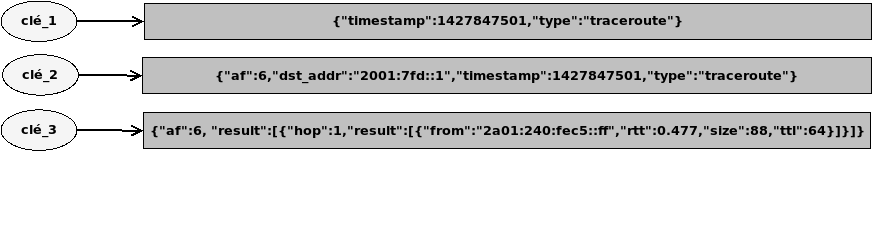
\includegraphics[width=1\linewidth]{illustrations/document-nosql}
			\caption{Illustration d'une base de données NoSQL de type document}
			\label{fig:document-nosql}
		\end{figure}
	

		\subparagraph{Colonnes} Dans les bases de données traditionnelles, les données sont stockées sur des lignes. Dans le cas d'une base NoSQL orientée colonne, les données sont stockées par colonne. L'interrogation de ce type de bases travaille sur une colonne particulière sans devoir passer par les autres colonnes comme dans les bases de données relationnelles classiques. Une base de données de type colonne, illustrée dans la Figure  	\ref{fig:comomn-nosql}, est adaptée pour les requêtes analytiques comme les requêtes d'agrégation (moyennes, maximum, etc).

	
	\begin{figure}[H]
		\centering
		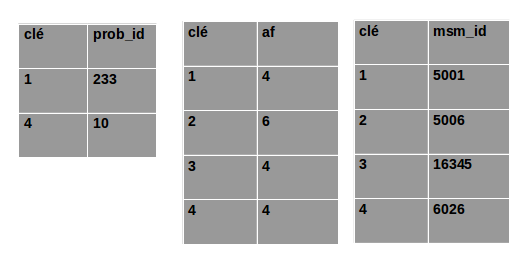
\includegraphics[width=0.7\linewidth]{illustrations/colomn-nosql.png}
		\caption{Illustration d'une base de données NoSQL de type colonne}
		\label{fig:comomn-nosql}
	\end{figure}
	

	\subparagraph{Graphe} Dans une base de données de type graphe, les données stockées sont les n\oe{}uds, les liens et les propriétés sur les n\oe{}uds et sur les liens. Un exemple  de base de données NoSQL de type graphe est le réseau social; chaque entité représente une personne et les relations entre ces personnes peuvent prendre plusieurs formes. Comme il est illustré dans la Figure  	\ref{fig:graphe-nosql}.

	
	\begin{figure}[H]
		\centering
		\resizebox{\textwidth}{!}{
		% Graphic for TeX using PGF
% Title: /home/hayat/report_memoire/illustrations/graphe-nosql.dia
% Creator: Dia v0.97+git
% CreationDate: Sun Dec  2 17:45:15 2018
% For: hayat
% \usepackage{tikz}
% The following commands are not supported in PSTricks at present
% We define them conditionally, so when they are implemented,
% this pgf file will use them.
\ifx\du\undefined
  \newlength{\du}
\fi
\setlength{\du}{15\unitlength}
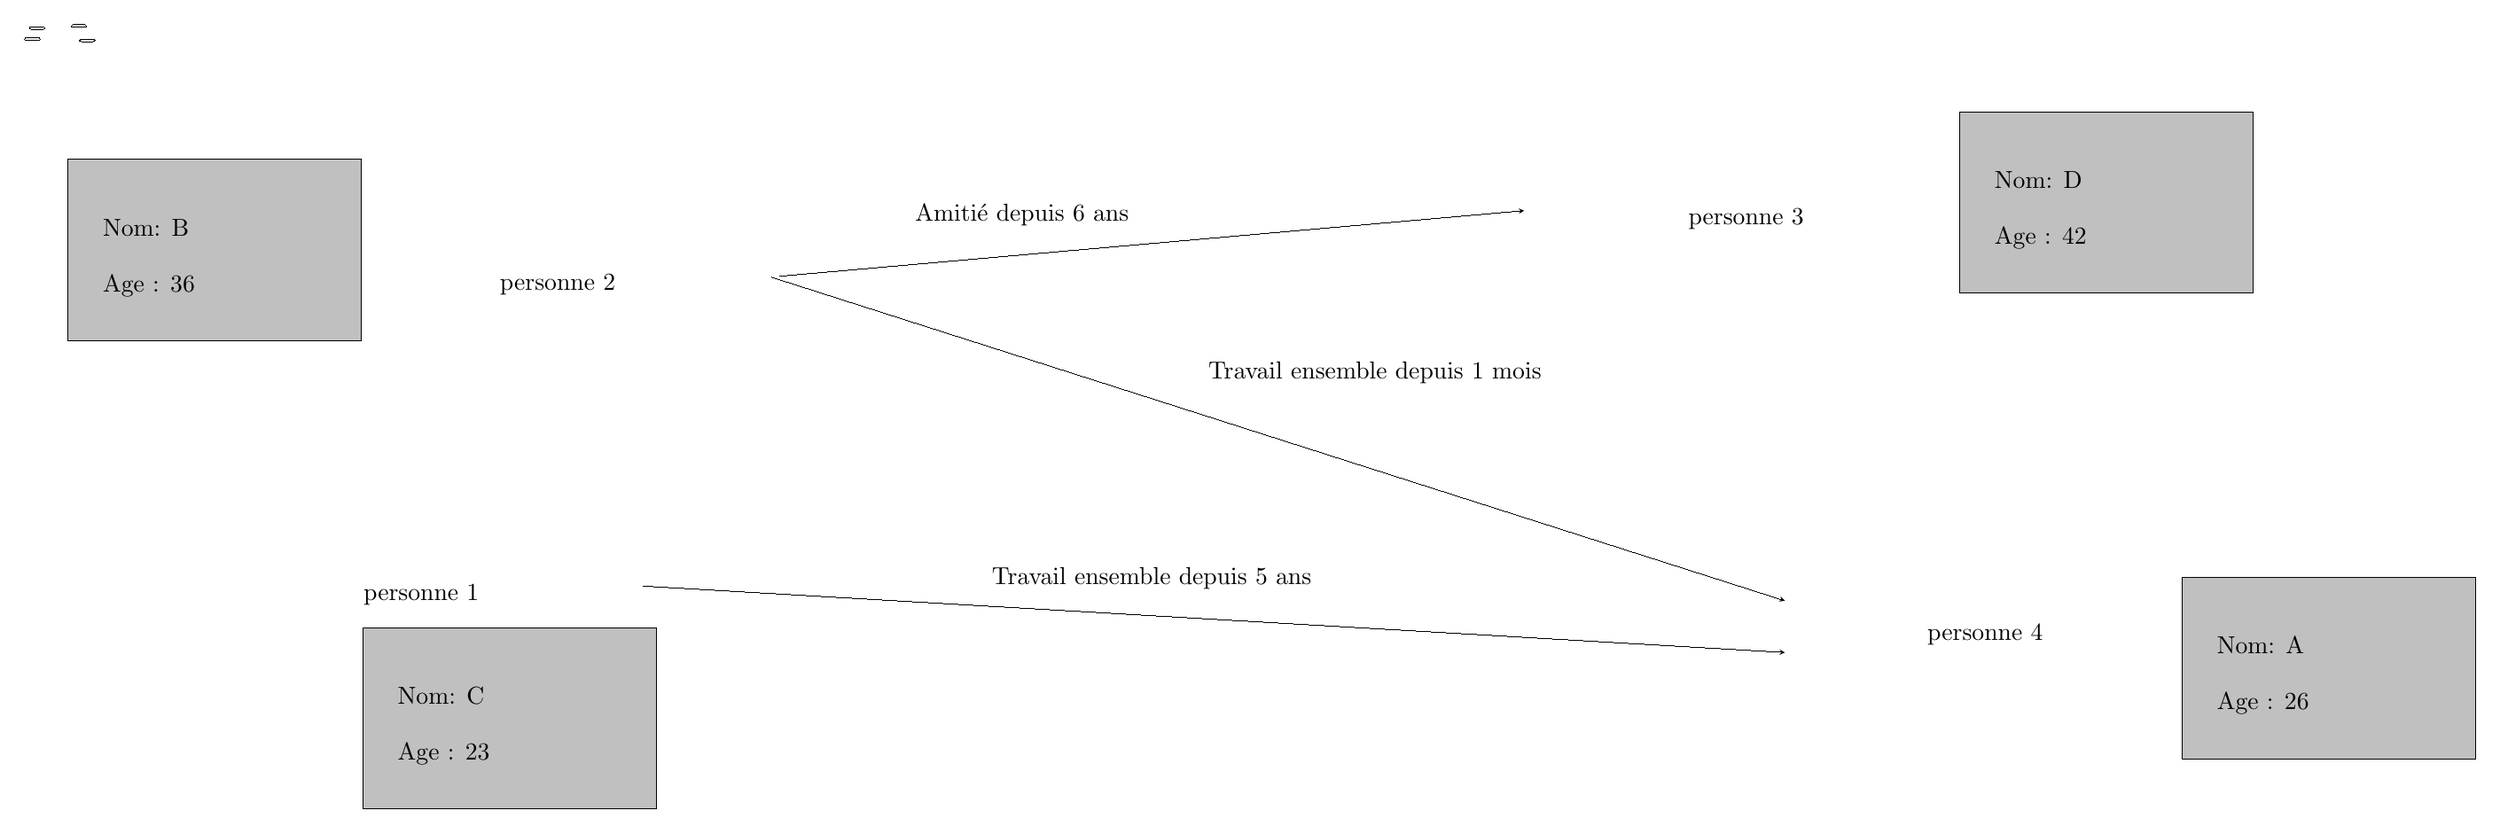
\begin{tikzpicture}[even odd rule]
\pgftransformxscale{1.000000}
\pgftransformyscale{-1.000000}
\definecolor{dialinecolor}{rgb}{0.000000, 0.000000, 0.000000}
\pgfsetstrokecolor{dialinecolor}
\pgfsetstrokeopacity{1.000000}
\definecolor{diafillcolor}{rgb}{1.000000, 1.000000, 1.000000}
\pgfsetfillcolor{diafillcolor}
\pgfsetfillopacity{1.000000}
\pgfsetlinewidth{0.000000\du}
\pgfsetdash{}{0pt}
\pgfsetbuttcap
\pgfsetmiterjoin
\pgfsetlinewidth{0.000000\du}
\pgfsetbuttcap
\pgfsetmiterjoin
\pgfsetdash{}{0pt}
\definecolor{diafillcolor}{rgb}{0.960784, 0.960784, 0.960784}
\pgfsetfillcolor{diafillcolor}
\pgfsetfillopacity{1.000000}
\definecolor{dialinecolor}{rgb}{0.000000, 0.000000, 0.000000}
\pgfsetstrokecolor{dialinecolor}
\pgfsetstrokeopacity{1.000000}
\pgfpathmoveto{\pgfpoint{3.655000\du}{7.600000\du}}
\pgfpathlineto{\pgfpoint{7.895000\du}{7.600000\du}}
\pgfpathcurveto{\pgfpoint{8.480422\du}{7.600000\du}}{\pgfpoint{8.955000\du}{7.835050\du}}{\pgfpoint{8.955000\du}{8.125000\du}}
\pgfpathcurveto{\pgfpoint{8.955000\du}{8.414950\du}}{\pgfpoint{8.480422\du}{8.650000\du}}{\pgfpoint{7.895000\du}{8.650000\du}}
\pgfpathlineto{\pgfpoint{3.655000\du}{8.650000\du}}
\pgfpathcurveto{\pgfpoint{3.069578\du}{8.650000\du}}{\pgfpoint{2.595000\du}{8.414950\du}}{\pgfpoint{2.595000\du}{8.125000\du}}
\pgfpathcurveto{\pgfpoint{2.595000\du}{7.835050\du}}{\pgfpoint{3.069578\du}{7.600000\du}}{\pgfpoint{3.655000\du}{7.600000\du}}
\pgfpathclose
\pgfusepath{fill,stroke}
% setfont left to latex
\definecolor{dialinecolor}{rgb}{0.000000, 0.000000, 0.000000}
\pgfsetstrokecolor{dialinecolor}
\pgfsetstrokeopacity{1.000000}
\definecolor{diafillcolor}{rgb}{0.000000, 0.000000, 0.000000}
\pgfsetfillcolor{diafillcolor}
\pgfsetfillopacity{1.000000}
\node[anchor=base,inner sep=0pt, outer sep=0pt,color=dialinecolor] at (5.775000\du,8.325000\du){personne 1};
\pgfsetlinewidth{0.000000\du}
\pgfsetdash{}{0pt}
\pgfsetbuttcap
\pgfsetmiterjoin
\pgfsetlinewidth{0.000000\du}
\pgfsetbuttcap
\pgfsetmiterjoin
\pgfsetdash{}{0pt}
\definecolor{diafillcolor}{rgb}{0.960784, 0.960784, 0.960784}
\pgfsetfillcolor{diafillcolor}
\pgfsetfillopacity{1.000000}
\definecolor{dialinecolor}{rgb}{0.000000, 0.000000, 0.000000}
\pgfsetstrokecolor{dialinecolor}
\pgfsetstrokeopacity{1.000000}
\pgfpathmoveto{\pgfpoint{5.608750\du}{3.160000\du}}
\pgfpathlineto{\pgfpoint{9.848750\du}{3.160000\du}}
\pgfpathcurveto{\pgfpoint{10.434172\du}{3.160000\du}}{\pgfpoint{10.908750\du}{3.395050\du}}{\pgfpoint{10.908750\du}{3.685000\du}}
\pgfpathcurveto{\pgfpoint{10.908750\du}{3.974950\du}}{\pgfpoint{10.434172\du}{4.210000\du}}{\pgfpoint{9.848750\du}{4.210000\du}}
\pgfpathlineto{\pgfpoint{5.608750\du}{4.210000\du}}
\pgfpathcurveto{\pgfpoint{5.023328\du}{4.210000\du}}{\pgfpoint{4.548750\du}{3.974950\du}}{\pgfpoint{4.548750\du}{3.685000\du}}
\pgfpathcurveto{\pgfpoint{4.548750\du}{3.395050\du}}{\pgfpoint{5.023328\du}{3.160000\du}}{\pgfpoint{5.608750\du}{3.160000\du}}
\pgfpathclose
\pgfusepath{fill,stroke}
% setfont left to latex
\definecolor{dialinecolor}{rgb}{0.000000, 0.000000, 0.000000}
\pgfsetstrokecolor{dialinecolor}
\pgfsetstrokeopacity{1.000000}
\definecolor{diafillcolor}{rgb}{0.000000, 0.000000, 0.000000}
\pgfsetfillcolor{diafillcolor}
\pgfsetfillopacity{1.000000}
\node[anchor=base,inner sep=0pt, outer sep=0pt,color=dialinecolor] at (7.728750\du,3.885000\du){personne 2};
\pgfsetlinewidth{0.000000\du}
\pgfsetdash{}{0pt}
\pgfsetbuttcap
\pgfsetmiterjoin
\pgfsetlinewidth{0.000000\du}
\pgfsetbuttcap
\pgfsetmiterjoin
\pgfsetdash{}{0pt}
\definecolor{diafillcolor}{rgb}{0.960784, 0.960784, 0.960784}
\pgfsetfillcolor{diafillcolor}
\pgfsetfillopacity{1.000000}
\definecolor{dialinecolor}{rgb}{0.000000, 0.000000, 0.000000}
\pgfsetstrokecolor{dialinecolor}
\pgfsetstrokeopacity{1.000000}
\pgfpathmoveto{\pgfpoint{22.633750\du}{2.220000\du}}
\pgfpathlineto{\pgfpoint{26.873750\du}{2.220000\du}}
\pgfpathcurveto{\pgfpoint{27.459172\du}{2.220000\du}}{\pgfpoint{27.933750\du}{2.455050\du}}{\pgfpoint{27.933750\du}{2.745000\du}}
\pgfpathcurveto{\pgfpoint{27.933750\du}{3.034950\du}}{\pgfpoint{27.459172\du}{3.270000\du}}{\pgfpoint{26.873750\du}{3.270000\du}}
\pgfpathlineto{\pgfpoint{22.633750\du}{3.270000\du}}
\pgfpathcurveto{\pgfpoint{22.048328\du}{3.270000\du}}{\pgfpoint{21.573750\du}{3.034950\du}}{\pgfpoint{21.573750\du}{2.745000\du}}
\pgfpathcurveto{\pgfpoint{21.573750\du}{2.455050\du}}{\pgfpoint{22.048328\du}{2.220000\du}}{\pgfpoint{22.633750\du}{2.220000\du}}
\pgfpathclose
\pgfusepath{fill,stroke}
% setfont left to latex
\definecolor{dialinecolor}{rgb}{0.000000, 0.000000, 0.000000}
\pgfsetstrokecolor{dialinecolor}
\pgfsetstrokeopacity{1.000000}
\definecolor{diafillcolor}{rgb}{0.000000, 0.000000, 0.000000}
\pgfsetfillcolor{diafillcolor}
\pgfsetfillopacity{1.000000}
\node[anchor=base,inner sep=0pt, outer sep=0pt,color=dialinecolor] at (24.753750\du,2.945000\du){personne 3};
\pgfsetlinewidth{0.000000\du}
\pgfsetdash{}{0pt}
\pgfsetbuttcap
\pgfsetmiterjoin
\pgfsetlinewidth{0.000000\du}
\pgfsetbuttcap
\pgfsetmiterjoin
\pgfsetdash{}{0pt}
\definecolor{diafillcolor}{rgb}{0.960784, 0.960784, 0.960784}
\pgfsetfillcolor{diafillcolor}
\pgfsetfillopacity{1.000000}
\definecolor{dialinecolor}{rgb}{0.000000, 0.000000, 0.000000}
\pgfsetstrokecolor{dialinecolor}
\pgfsetstrokeopacity{1.000000}
\pgfpathmoveto{\pgfpoint{26.058750\du}{8.180000\du}}
\pgfpathlineto{\pgfpoint{30.298750\du}{8.180000\du}}
\pgfpathcurveto{\pgfpoint{30.884172\du}{8.180000\du}}{\pgfpoint{31.358750\du}{8.415050\du}}{\pgfpoint{31.358750\du}{8.705000\du}}
\pgfpathcurveto{\pgfpoint{31.358750\du}{8.994950\du}}{\pgfpoint{30.884172\du}{9.230000\du}}{\pgfpoint{30.298750\du}{9.230000\du}}
\pgfpathlineto{\pgfpoint{26.058750\du}{9.230000\du}}
\pgfpathcurveto{\pgfpoint{25.473328\du}{9.230000\du}}{\pgfpoint{24.998750\du}{8.994950\du}}{\pgfpoint{24.998750\du}{8.705000\du}}
\pgfpathcurveto{\pgfpoint{24.998750\du}{8.415050\du}}{\pgfpoint{25.473328\du}{8.180000\du}}{\pgfpoint{26.058750\du}{8.180000\du}}
\pgfpathclose
\pgfusepath{fill,stroke}
% setfont left to latex
\definecolor{dialinecolor}{rgb}{0.000000, 0.000000, 0.000000}
\pgfsetstrokecolor{dialinecolor}
\pgfsetstrokeopacity{1.000000}
\definecolor{diafillcolor}{rgb}{0.000000, 0.000000, 0.000000}
\pgfsetfillcolor{diafillcolor}
\pgfsetfillopacity{1.000000}
\node[anchor=base,inner sep=0pt, outer sep=0pt,color=dialinecolor] at (28.178750\du,8.905000\du){personne 4};
\pgfsetlinewidth{0.000000\du}
\pgfsetdash{}{0pt}
\pgfsetbuttcap
{
\definecolor{diafillcolor}{rgb}{0.000000, 0.000000, 0.000000}
\pgfsetfillcolor{diafillcolor}
\pgfsetfillopacity{1.000000}
% was here!!!
\pgfsetarrowsend{stealth}
\definecolor{dialinecolor}{rgb}{0.000000, 0.000000, 0.000000}
\pgfsetstrokecolor{dialinecolor}
\pgfsetstrokeopacity{1.000000}
\draw (10.908750\du,3.685000\du)--(21.573750\du,2.745000\du);
}
% setfont left to latex
\definecolor{dialinecolor}{rgb}{0.000000, 0.000000, 0.000000}
\pgfsetstrokecolor{dialinecolor}
\pgfsetstrokeopacity{1.000000}
\definecolor{diafillcolor}{rgb}{0.000000, 0.000000, 0.000000}
\pgfsetfillcolor{diafillcolor}
\pgfsetfillopacity{1.000000}
\node[anchor=base west,inner sep=0pt,outer sep=0pt,color=dialinecolor] at (12.850000\du,2.900000\du){Amitié depuis 6 ans};
\pgfsetlinewidth{0.000000\du}
\pgfsetdash{}{0pt}
\pgfsetbuttcap
{
\definecolor{diafillcolor}{rgb}{0.000000, 0.000000, 0.000000}
\pgfsetfillcolor{diafillcolor}
\pgfsetfillopacity{1.000000}
% was here!!!
\pgfsetarrowsend{stealth}
\definecolor{dialinecolor}{rgb}{0.000000, 0.000000, 0.000000}
\pgfsetstrokecolor{dialinecolor}
\pgfsetstrokeopacity{1.000000}
\draw (8.955000\du,8.125000\du)--(25.309224\du,9.076227\du);
}
% setfont left to latex
\definecolor{dialinecolor}{rgb}{0.000000, 0.000000, 0.000000}
\pgfsetstrokecolor{dialinecolor}
\pgfsetstrokeopacity{1.000000}
\definecolor{diafillcolor}{rgb}{0.000000, 0.000000, 0.000000}
\pgfsetfillcolor{diafillcolor}
\pgfsetfillopacity{1.000000}
\node[anchor=base west,inner sep=0pt,outer sep=0pt,color=dialinecolor] at (13.950000\du,8.100000\du){Travail ensemble depuis 5 ans};
\pgfsetlinewidth{0.000000\du}
\pgfsetdash{}{0pt}
\pgfsetbuttcap
{
\definecolor{diafillcolor}{rgb}{0.000000, 0.000000, 0.000000}
\pgfsetfillcolor{diafillcolor}
\pgfsetfillopacity{1.000000}
% was here!!!
\pgfsetarrowsend{stealth}
\definecolor{dialinecolor}{rgb}{0.000000, 0.000000, 0.000000}
\pgfsetstrokecolor{dialinecolor}
\pgfsetstrokeopacity{1.000000}
\draw (10.800000\du,3.700000\du)--(25.309224\du,8.333773\du);
}
% setfont left to latex
\definecolor{dialinecolor}{rgb}{0.000000, 0.000000, 0.000000}
\pgfsetstrokecolor{dialinecolor}
\pgfsetstrokeopacity{1.000000}
\definecolor{diafillcolor}{rgb}{0.000000, 0.000000, 0.000000}
\pgfsetfillcolor{diafillcolor}
\pgfsetfillopacity{1.000000}
\node[anchor=base west,inner sep=0pt,outer sep=0pt,color=dialinecolor] at (17.050000\du,5.150000\du){Travail ensemble depuis 1 mois};
\pgfsetlinewidth{0.000000\du}
\pgfsetdash{}{0pt}
\pgfsetmiterjoin
{\pgfsetcornersarced{\pgfpoint{0.000000\du}{0.000000\du}}\definecolor{diafillcolor}{rgb}{0.752941, 0.752941, 0.752941}
\pgfsetfillcolor{diafillcolor}
\pgfsetfillopacity{1.000000}
\fill (31.000050\du,8.000000\du)--(31.000050\du,10.600000\du)--(35.200050\du,10.600000\du)--(35.200050\du,8.000000\du)--cycle;
}{\pgfsetcornersarced{\pgfpoint{0.000000\du}{0.000000\du}}\definecolor{dialinecolor}{rgb}{0.000000, 0.000000, 0.000000}
\pgfsetstrokecolor{dialinecolor}
\pgfsetstrokeopacity{1.000000}
\draw (31.000050\du,8.000000\du)--(31.000050\du,10.600000\du)--(35.200050\du,10.600000\du)--(35.200050\du,8.000000\du)--cycle;
}% setfont left to latex
\definecolor{dialinecolor}{rgb}{0.000000, 0.000000, 0.000000}
\pgfsetstrokecolor{dialinecolor}
\pgfsetstrokeopacity{1.000000}
\definecolor{diafillcolor}{rgb}{0.000000, 0.000000, 0.000000}
\pgfsetfillcolor{diafillcolor}
\pgfsetfillopacity{1.000000}
\node[anchor=base west,inner sep=0pt,outer sep=0pt,color=dialinecolor] at (31.500050\du,9.095000\du){Nom: A};
% setfont left to latex
\definecolor{dialinecolor}{rgb}{0.000000, 0.000000, 0.000000}
\pgfsetstrokecolor{dialinecolor}
\pgfsetstrokeopacity{1.000000}
\definecolor{diafillcolor}{rgb}{0.000000, 0.000000, 0.000000}
\pgfsetfillcolor{diafillcolor}
\pgfsetfillopacity{1.000000}
\node[anchor=base west,inner sep=0pt,outer sep=0pt,color=dialinecolor] at (31.500050\du,9.895000\du){Age : 26 };
\pgfsetlinewidth{0.000000\du}
\pgfsetdash{}{0pt}
\pgfsetmiterjoin
{\pgfsetcornersarced{\pgfpoint{0.000000\du}{0.000000\du}}\definecolor{diafillcolor}{rgb}{0.752941, 0.752941, 0.752941}
\pgfsetfillcolor{diafillcolor}
\pgfsetfillopacity{1.000000}
\fill (0.713750\du,2.010000\du)--(0.713750\du,4.610000\du)--(4.913750\du,4.610000\du)--(4.913750\du,2.010000\du)--cycle;
}{\pgfsetcornersarced{\pgfpoint{0.000000\du}{0.000000\du}}\definecolor{dialinecolor}{rgb}{0.000000, 0.000000, 0.000000}
\pgfsetstrokecolor{dialinecolor}
\pgfsetstrokeopacity{1.000000}
\draw (0.713750\du,2.010000\du)--(0.713750\du,4.610000\du)--(4.913750\du,4.610000\du)--(4.913750\du,2.010000\du)--cycle;
}% setfont left to latex
\definecolor{dialinecolor}{rgb}{0.000000, 0.000000, 0.000000}
\pgfsetstrokecolor{dialinecolor}
\pgfsetstrokeopacity{1.000000}
\definecolor{diafillcolor}{rgb}{0.000000, 0.000000, 0.000000}
\pgfsetfillcolor{diafillcolor}
\pgfsetfillopacity{1.000000}
\node[anchor=base west,inner sep=0pt,outer sep=0pt,color=dialinecolor] at (1.213750\du,3.105000\du){Nom: B};
% setfont left to latex
\definecolor{dialinecolor}{rgb}{0.000000, 0.000000, 0.000000}
\pgfsetstrokecolor{dialinecolor}
\pgfsetstrokeopacity{1.000000}
\definecolor{diafillcolor}{rgb}{0.000000, 0.000000, 0.000000}
\pgfsetfillcolor{diafillcolor}
\pgfsetfillopacity{1.000000}
\node[anchor=base west,inner sep=0pt,outer sep=0pt,color=dialinecolor] at (1.213750\du,3.905000\du){Age : 36 };
\pgfsetlinewidth{0.000000\du}
\pgfsetdash{}{0pt}
\pgfsetmiterjoin
{\pgfsetcornersarced{\pgfpoint{0.000000\du}{0.000000\du}}\definecolor{diafillcolor}{rgb}{0.752941, 0.752941, 0.752941}
\pgfsetfillcolor{diafillcolor}
\pgfsetfillopacity{1.000000}
\fill (4.938750\du,8.720000\du)--(4.938750\du,11.320000\du)--(9.138750\du,11.320000\du)--(9.138750\du,8.720000\du)--cycle;
}{\pgfsetcornersarced{\pgfpoint{0.000000\du}{0.000000\du}}\definecolor{dialinecolor}{rgb}{0.000000, 0.000000, 0.000000}
\pgfsetstrokecolor{dialinecolor}
\pgfsetstrokeopacity{1.000000}
\draw (4.938750\du,8.720000\du)--(4.938750\du,11.320000\du)--(9.138750\du,11.320000\du)--(9.138750\du,8.720000\du)--cycle;
}% setfont left to latex
\definecolor{dialinecolor}{rgb}{0.000000, 0.000000, 0.000000}
\pgfsetstrokecolor{dialinecolor}
\pgfsetstrokeopacity{1.000000}
\definecolor{diafillcolor}{rgb}{0.000000, 0.000000, 0.000000}
\pgfsetfillcolor{diafillcolor}
\pgfsetfillopacity{1.000000}
\node[anchor=base west,inner sep=0pt,outer sep=0pt,color=dialinecolor] at (5.438750\du,9.815000\du){Nom: C};
% setfont left to latex
\definecolor{dialinecolor}{rgb}{0.000000, 0.000000, 0.000000}
\pgfsetstrokecolor{dialinecolor}
\pgfsetstrokeopacity{1.000000}
\definecolor{diafillcolor}{rgb}{0.000000, 0.000000, 0.000000}
\pgfsetfillcolor{diafillcolor}
\pgfsetfillopacity{1.000000}
\node[anchor=base west,inner sep=0pt,outer sep=0pt,color=dialinecolor] at (5.438750\du,10.615000\du){Age : 23 };
\pgfsetlinewidth{0.000000\du}
\pgfsetdash{}{0pt}
\pgfsetmiterjoin
{\pgfsetcornersarced{\pgfpoint{0.000000\du}{0.000000\du}}\definecolor{diafillcolor}{rgb}{0.752941, 0.752941, 0.752941}
\pgfsetfillcolor{diafillcolor}
\pgfsetfillopacity{1.000000}
\fill (27.813750\du,1.330000\du)--(27.813750\du,3.930000\du)--(32.013750\du,3.930000\du)--(32.013750\du,1.330000\du)--cycle;
}{\pgfsetcornersarced{\pgfpoint{0.000000\du}{0.000000\du}}\definecolor{dialinecolor}{rgb}{0.000000, 0.000000, 0.000000}
\pgfsetstrokecolor{dialinecolor}
\pgfsetstrokeopacity{1.000000}
\draw (27.813750\du,1.330000\du)--(27.813750\du,3.930000\du)--(32.013750\du,3.930000\du)--(32.013750\du,1.330000\du)--cycle;
}% setfont left to latex
\definecolor{dialinecolor}{rgb}{0.000000, 0.000000, 0.000000}
\pgfsetstrokecolor{dialinecolor}
\pgfsetstrokeopacity{1.000000}
\definecolor{diafillcolor}{rgb}{0.000000, 0.000000, 0.000000}
\pgfsetfillcolor{diafillcolor}
\pgfsetfillopacity{1.000000}
\node[anchor=base west,inner sep=0pt,outer sep=0pt,color=dialinecolor] at (28.313750\du,2.425000\du){Nom: D};
% setfont left to latex
\definecolor{dialinecolor}{rgb}{0.000000, 0.000000, 0.000000}
\pgfsetstrokecolor{dialinecolor}
\pgfsetstrokeopacity{1.000000}
\definecolor{diafillcolor}{rgb}{0.000000, 0.000000, 0.000000}
\pgfsetfillcolor{diafillcolor}
\pgfsetfillopacity{1.000000}
\node[anchor=base west,inner sep=0pt,outer sep=0pt,color=dialinecolor] at (28.313750\du,3.225000\du){Age : 42 };
\end{tikzpicture}

	    }
		\caption{Illustration d'une base de données NoSQL de type graphe}
		\label{fig:graphe-nosql}
	\end{figure}
	
	Il existe plusieurs implémentations des quatre types de bases de données NoSQL. Chaque implémentation favorise un ou plus des éléments suivants : la disponibilité des données, la cohérence des données et la tolérance au partitionnement.  C'est ce qu'explique le théorème CAP.	
		
		\paragraph{Big Data et le théorème  CAP} \label{par:cap-theorem}:
		
		Dans le but d'assurer un traitement rapide de données à grande échelle, ces dernières sont répartie sur un nombre de machines  (ou n\oe{}uds). Le théorème CAP annonce que dans le cadre d'un système distribué où les données sont réparties sur plusieurs machines,
		%(ou n\oe{}uds) (voir \ref{sec:distruted-camput}),  
		une base de données ne peut pas garantir les trois attributs suivants: \textit{Consistency}, \textit{Availability}, et \textit{Partition Tolerence}  en même temps. 
		
		
			\subparagraph{ Consistency (ou intégrité)} Chaque donnée a un seul état visible depuis l'extérieur. Par exemple, les différents serveurs hébergeant la base de données voient tous les mêmes données. C'est pourquoi une lecture faite après une écriture doit renvoyer la donnée précédemment écrite.
			
			\subparagraph{ Availability (ou disponibilité)} Une base de données doit toujours fournir une réponse à une requête d'un client.
			
			%En cas d'une panne technique sur un des serveurs qui hébergent  la base de données, il faut s'assurer de desservir  des clients.  Généralement, cela est assuré à travers la réplication des données
			
			 \subparagraph{Partition tolerance (ou la tolérance au partitionnement) } Une coupure du réseau entre deux n\oe{}uds ou l'indisponibilité d'un de ces n\oe{}uds ne devrait pas affecter le bon fonctionnement du système. Tout de même,  ce dernier doit répondre à la demande d'un client. 

		
		%conclusion
		Les trois attributs du théorème CAP s'opposent entre eux. On distingue les trois scénarios possibles:
		
		\begin{itemize}
			\item [--] Le couple \textbf{CA} : les SGBDR adoptent les deux attributs C et A, qui sont une forte cohérence et disponibilité. Cependant, l'attribut partitionnement réseau n'est pas toujours pris en compte.
			\item [--] Le couple \textbf{CP} : les implémentations du C et du P assurent la tolérance aux pannes en distribuant les données sur plusieurs serveurs. Malgré cette réplication, ces implémentations assurent la cohérence des données même en présence de mises à jour concurrentielles.
			\item [--] Le couple \textbf{AP} : les implémentations du A et du  P assurent un temps de réponse rapide et une réplication des données. Cependant, les mises à jour étant asynchrones, la garantie que la version d'une donnée soit bonne, ne peut pas être assurée.
			
		\end{itemize}
		
		La Figure \ref{fig:cap} présente des implémentations des différents types de bases de données NoSQL pour chaque couple CA, CP et AP.
		
		\begin{figure}[H]
			\centering
			\captionsetup{justification=centering}
			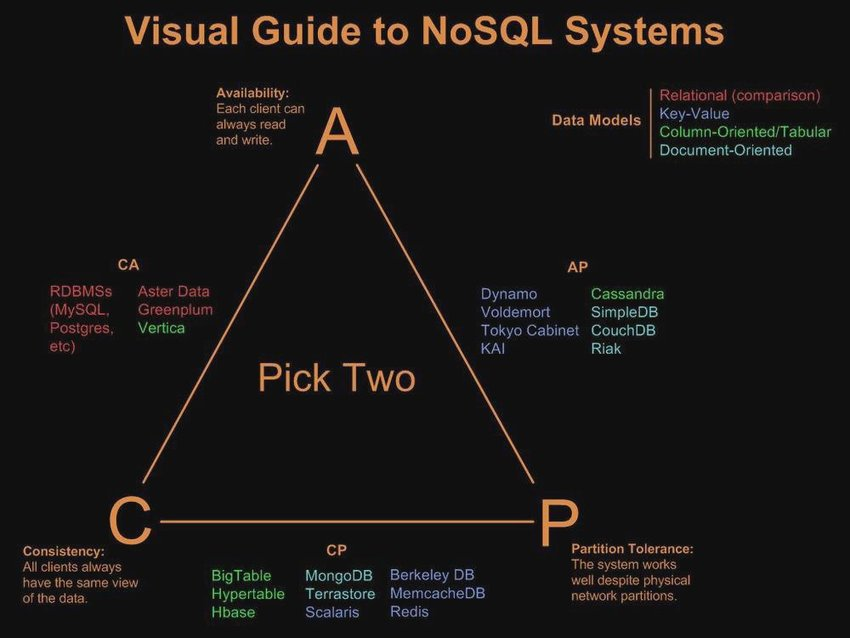
\includegraphics[width=1\linewidth]{illustrations/cap}
			\caption{Bases de données NoSQL suivant le théorème de CAP }
			\label{fig:cap}
			\source{\url{https://payberah.github.io/files/download/p2p/nosql.pdf}, consultée le $05/08/2018$.}
		\end{figure}
		
		
		
		Le choix d'une base de données relationnelle ou NoSQL dépend des besoins des entreprises. En terme de tendances, la Figure \ref{fig:ranking-db} reprend un classement des SGBDs au $1$ août $ 2018 $. La suite de la liste ainsi que  la méthode qui dirige ce classement sont    disponibles sur le site  web \textit{DB-Engines Ranking}\footnote{Source : \url{https://db-engines.com/},  consultée le $01/08/2018$.}. Parmi les critères du classement, on trouve le nombre de références du SGBD sur les sites Internet. 
		
		%Ce nombre de référence est quantifiable à partir du  nombre lui-même de résultats obtenus des différents moteurs de recherche comme Google, Bing, etc. 
		
		\begin{figure}[H]
			\centering
			\captionsetup{justification=centering}
			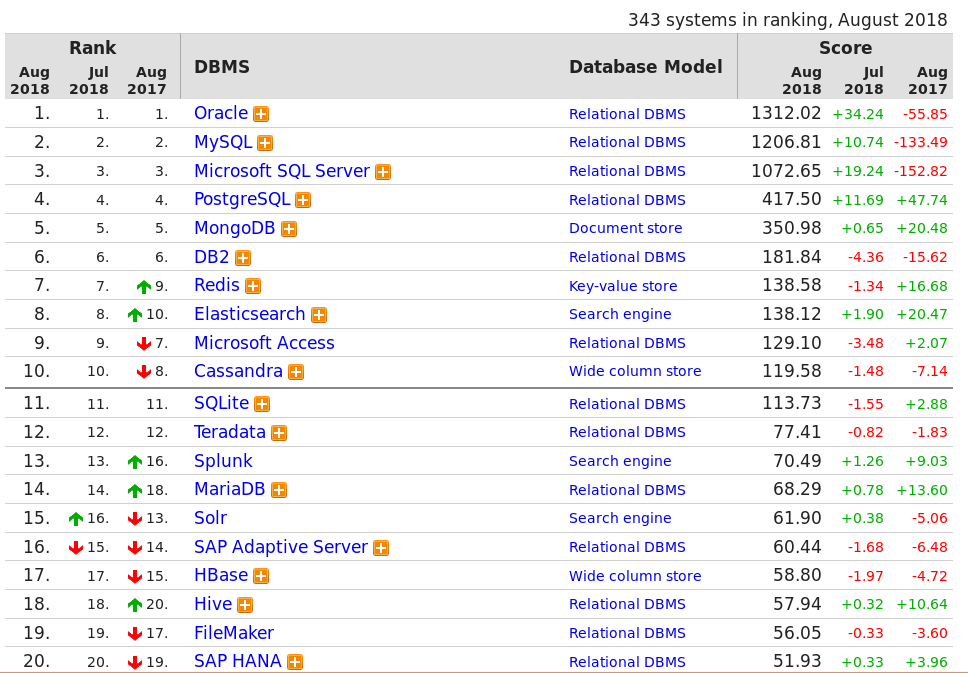
\includegraphics[width=1\linewidth]{illustrations/ranking-db}
			\caption{Un classement des SGBDs sur \textit{DB-Engines Ranking} du $1$ août $2018$ }
			\label{fig:ranking-db}
			\source{\url{https://db-engines.com/en/ranking}, consultée le $01/08/2018$.}
		\end{figure}
		
		
		
		\subsection{Schema on Write VS Schema on Read} \label{sec:schema-read-write}
		
		Lors du chargement des données depuis leurs sources de stockage, on distingue deux approches : \textit{ Schema on Write} et \textit{Schema on Read}.
		% L'approche \textit{Schema on Read } est celle utilisée par l'outil Amazon Athena présenté dans la section \ref{par:allservices}.
		
		Dans la première, il faut définir les colonnes, le format de données, les types, etc. La lecture des données est rapide et moins coûteuse étant donné l'effort entreprit pour définir la structure. C'est le cas des bases de données relationnelles.
		
		Dans la deuxième, les données sont chargées telles qu'elles sont, sans transformations ou changements. L'interprétation de ces données se fait lors de la lecture, et cela dépend des besoins pour lesquels les données sont analysées. Ainsi, les mêmes données peuvent être lues de différentes manières. Par exemple, l'action  de lire les données  d'une colonne, qu'elles soient de type entier ou bien chaîne de caractère d'un fichier CSV est la même, mais le type de la donnée qui diffère. C'est l'approche utilisée par Amazon Athena (voir \ref{aws:athena}). Les Figures \ref{fig:on-write} et \ref{fig:on-read} illustrent la différence entre ces deux approches.
		\begin{figure}[H]
			\centering
			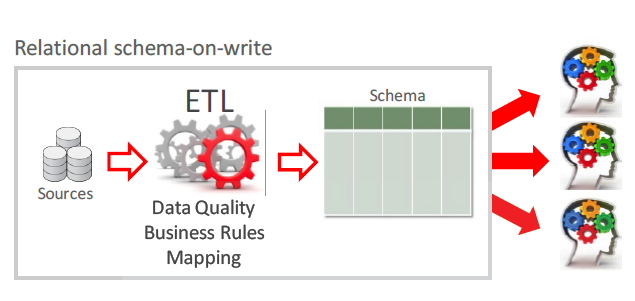
\includegraphics[width=0.8\linewidth]{illustrations/on-write}
			\caption{Schema on Write (SGBDR)}
			\label{fig:on-write}
		\end{figure}
		\begin{figure}[H]
			\centering
			\captionsetup{justification=centering}
			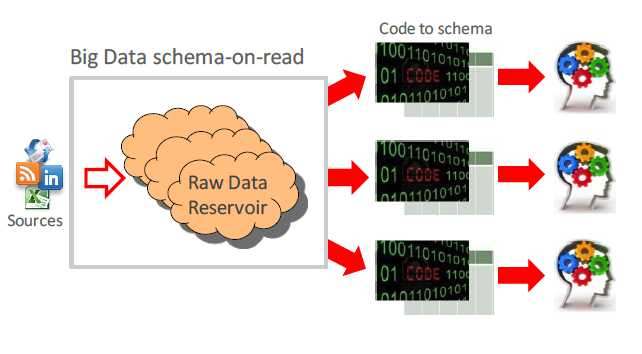
\includegraphics[width=0.8\linewidth]{illustrations/on-read}
			\caption{Schema on Read (Big Data)}
			\label{fig:on-read}
			\source{ \url{https://blogs.oracle.com/datawarehousing/big-data-sql-quick-start-schema-on-read-and-schema-on-write-part11}, consultée le $05/08/2018$.}
		\end{figure}
		
		La meilleure approche dépend des besoins de l'analyse. La première approche est meilleure en performances, en revanche, la deuxième est tolérante aux erreurs  humaines.
		
		
		\subsection{L'informatique distribuée et l'analyse de données massives} \label{sec:distruted-camput}
		Il existe deux stratégies pour appliquer des traitements sur un grand ensemble de données: 
		
		
		\begin{itemize}
			\item[--] Par distribution des traitements (\textit{scaling} des traitements)~: les traitements sont distribués sur un nombre de n\oe{}uds important. De ce fait, les données sont amenées jusqu'à ces n\oe{}uds;
			
			\item[--] Par distribution des données (\textit{scaling} des données)~: les données sont distribuées sur un nombre important de n\oe{}uds. D'ailleurs cela permet  de stocker un maximum de données. Il s'agit d'amener les traitements aux machines sur lesquelles les données sont stockées. Du fait que le stockage de données est réparti sur plusieurs machines, il est possible de traiter des données très volumineuses en un temps optimal. La première mise en \oe{}uvre de cette approche est le schéma Map-Reduce. 
		\end{itemize}
	
	\begin{tcolorbox}
	\textit{ MapReduce est un patron d'architecture de développement informatique, inventé par Google, dans lequel sont effectués des calculs parallèles, et souvent distribués, de données potentiellement très volumineuses, typiquement supérieures en taille à 1 téraoctet} \footnote{Source : \url{https://fr.wikipedia.org/wiki/MapReduce}, consultée le $20/12/2018$.}. 
	\end{tcolorbox}
	\section{Parcours de quelques technologies du Big Data}
	
La liste des technologies dans le domaine du Big Data est en expansion continue pour répondre au mieux aux besoins de l'analyse de données massives. C'est pourquoi nous allons parcourir une liste non exhaustive des technologies liées au Big Data. En particulier, ce sont les technologies expérimentées pour analyser les traceroutes en provenance du RIPE Atlas.
	
	\subsection{MongoDB} \label{subsubsection:mongodb}
	
	
%	\paragraph{Introduction à la base de données MongoDB} \label{subsubsection:mongodb}~
	
	MongoDB\footnote{Source : \url{https://www.mongodb.com/}, consultée le $02/08/2018$.} est une base de données  NoSQL de type Document\footnote{Une base de données NoSQL de type document est décrite dans la section \ref{sec:nosql-database}.}.  MongoDB est classé parmi les  SGBDs adoptant le couple CP (Consistency et Partition Tolerance) dans le théorème  CAP\footnote{Le théorème  CAP est décrit dans la section \ref{par:cap-theorem}}. Une base de données créées dans MongoDB est un ensemble de collections. Une collection dans MongoDB est équivalente à une table dans un SGBDR.
	
	En $ 2016 $, MongoDB devient disponible en mode cloud sous le nom  MongoDB Atlas \footnote{Source : \url{https://www.mongodb.com/cloud/atlas}, consultée le $ 02/08/2018 $.}.  Il est distribué à travers les trois fournisseurs du cloud: Amazon Web Services (AWS), Google Cloud Platform et Microsoft Azure.  En terme de tarifs, plusieurs formules sont proposées \footnote{Source : \url{https://www.mongodb.com/cloud/atlas/pricing}, consultée le $ 02/08/2018 $.}, y inclut l'offre gratuite pour expérimenter MongoDB Atlas.  Les frais d'utilisation du service MongoDB Atlas dépend du stockage, de la  RAM allouées et des options choisies. Les documents sont stockés dans MongoDB sous format BSON.
	
	 \begin{tcolorbox}
		BSON (ou Binary JSON) est un format utilisé pour stocker et transférer les données dans la base de données MongoDB. BSON facilite la représentation des structures de données simples et des tableaux associatifs\footnote{Source : \url{https://fr.wikipedia.org/wiki/BSON}, consultée le $ 02/08/2018 $.}.
	\end{tcolorbox}
	
	\subsection{Amazon DynamoDB}\label{aws:dynmo}~
	
	% \paragraph{Amazon DynamoDB :}\label{aws:dynmo}~
	
	Amazon DynamoDB\footnote{Source : \url{https://aws.amazon.com/fr/dynamodb/}, consultée le $02/05/2018$.} est une base de données NoSQL de type clé-valeur distribuée, gérée par les services d'Amazon. Elle est capable de stocker un volume important de données limité par la capacité de l'infrastructure d'AWS. Amazon DynamoDB   est un service  simple et facile à utiliser,  il ne nécessite aucune configuration préalable. 
	
	Amazon DynamoDB  est une base de données évolutive de façon abstraite pour l'utilisateur final. Elle offre des performances constantes à une échelle essentiellement infinie, limitée uniquement par la taille physique du cloud AWS. Elle est flexible. Aucun schéma n'est requis pour stocker les données. Les frais d'utilisation de ce service dépendent de trois éléments\footnote{Source : \url{https://aws.amazon.com/fr/dynamodb/pricing/}, consultée $02/05/2018$.}:
	\begin{itemize}
		\item[--] la quantité de données stockées : DynamoDB est facturé par Go d'espace disque utilisé ($ 0,250 $ USD par Go par mois);
		\item[--] la capacité en lecture par seconde ($ 0,470 $ USD par unité de capacité d'écriture par mois);
		\item[--]  la capacité en écriture par seconde ($ 0,090 $ USD par unité de capacité de lecture par mois);
	\end{itemize}

\subsection{Amazon S3, Amazon Glue et Amazon Athena }

La combinaison d'Amazon S3, Amazon Glue et Amazon Athena permet de créer un environnement Big Data capable d'assurer le stockage de données, le chargement de données  et l'interrogation de données. 

%\paragraph{Introduction aux services Amazon S3, Amazon Athena et Amazon Glue }

\paragraph{Amazon S3}
\footnote{Source : \url{https://aws.amazon.com/fr/s3/}, consultée le $06/07/2018$.} est un service de stockage d'objets dans le cloud. Il est conçu pour stocker et  récupérer toute quantité de données. Il peut assurer $ 99,999999999 $ \% de durabilité. La sécurité  et l'accès aux données sont assurés. Il existe plusieurs classes de stockage qui répondent aux différents besoins. 


Les fichiers des données sont organisés dans ce qu'on appelle un compartiment, c'est une simulation de dossier dans un système d'exploitation. A l'intérieur d'un compartiment, il est possible de créer des compartiments imbriqués. C'est une simulation d'arborescence de dossiers car physiquement cet arborescence n'existe pas. En ce qui concerne les frais du service AWS S3, le Tableau   	\ref{tab:pricing-s3-standard} décrit les tarifs de la formule standard.
\begin{table}[H]
	\centering
	\captionsetup{justification=centering}
	\begin{tabular}{l c }
		\textbf{Région} & UE (Irlande) \\ \hline
		\textbf{Première tranche de $ 50 $ To/mois} &	$ 0,023 $ USD par Go\\ \hline
		\textbf{$ 450 $ To suivants/mois} &	$ 0,022 $ USD par Go \\ \hline
		\textbf{Plus de $ 500 $ To/mois} &	$ 0,021 $ USD par Go\\ \hline
	\end{tabular}
	\caption{Les tarifs du AWS S3 (formule Stockage standard S3)}
	\label{tab:pricing-s3-standard}
	\source{\url{https://aws.amazon.com/fr/s3/pricing/}, consultée le $05/08/2018$.}
\end{table}


\paragraph{Amazon  Glue} \label{aws:glue}
\footnote{Source : \url{https://aws.amazon.com/fr/glue/}, consultée le $06/07/2018$.} est un service d'extraction, de transformation et de chargement. L'objectif de ce service est de découvrir les données, les transformer et les rendre accessibles à la recherche et à l'interrogation.  Amazon Glue  est utile pour la construction des entrepôts de données; il découvre les métadonnées relatives aux magasins de données et les rendre accessibles dans un catalogue central. En prenant en entrée les données  présentes dans un compartiment dans Amazon S3, Amazon Glue découvre le schéma de ces données. Il dispose de plusieurs classificateurs intégrés pour la découverte des données. Par exemple un classificateur pour trouver le schéma  de données en format JSON, XML, etc. Si les classificateurs intégrés ne répondent pas aux besoins particuliers, il est possible de créer des classificateurs personnalisables. 

Les frais de ce service dépendent du temps écoulé lors de l'analyse des données par les robots d'analyse durant la découverte du schéma. A ces frais, ils s'ajoutent les frais du catalogue de données qui va être peuplé par les résultats fournis par les robots de l'analyse. Par exemple, on paye $ 0,44 $ USD par heure par DPU\footnote{DPU : unité de traitement des données.}, il est facturé à la seconde avec un minimum de $ 10 $ minutes par robot d'analyse exécuté. Plus de détails sont disponibles sur Amazon Glue\footnote{Source : \url{https://aws.amazon.com/fr/glue/pricing/}, consultée le $05/08/2018$.}.

\paragraph{Amazon Athena}\label{aws:athena}\footnote{Source : \url{https://aws.amazon.com/fr/athena/}, consultée le $06/07/2018$.} est un service de requêtes  interactif. Il permet d'interroger les données présentes dans Amazon S3 avec des requêtes SQL plus avancées. Le service Amazon Athena est considéré comme \textit{serverless}. Amazon Athena utilise l'approche \textbf{\textit{schema-on-read}} (voir la section \ref{sec:schema-read-write}) afin de projeter le schéma donné en entrée sur les données au moment de l'exécution de la requête SQL demandée. Le schéma sur lequel les données peuvent être projetées peut être créé manuellement ou bien utiliser le catalogue créé dans Amazon Glue.
Le service Amazon Athena est facturé suivant la quantité de données analysée. Précisément, $ 5 $ USD par To de données analysées.


\begin{tcolorbox}
	Une \textbf{\textit{requête est	interactive}} si on peut  obtenir immédiatement une réponse à la requête.  Dans le cas échéant, les résultats sont obtenus  dans le cadre d'un code source pour un des langages de programmation, souvent à travers une API.
\end{tcolorbox}

\begin{tcolorbox}
	\textbf{\textit{Serverless}} peut être décomposé en \textit{server} et \textit{less}. Un outil est \textit{serverless} quand l'utilisateur final de cet outil peut l'utiliser sans se soucier de toute configuration ou gestion des serveurs derrière ce service. C'est un mécanisme présent beaucoup sur le cloud.
\end{tcolorbox}

L'exécution des requêtes SQL est effectuée par le moteur de requêtes SQL Presto. pour les instruction DDL, elles sont effectuées par  \textit{Hive Data Definition Language} \footnote{Source : \url{https://cwiki.apache.org/confluence/display/Hive/LanguageManual+DDL}, consultée le $05/08/2018$.}. Les requêtes DDL incluent la création, la suppression et la mise à jour de la structure de la table dans le cas d'une base de données relationnelles, d'une collection, d'une vue, etc. 



\begin{tcolorbox}
	\textbf{\textit{Presto\footnote{Source : \url{http://prestodb.io/}, consultée le $01/08/2018$.} }} est un moteur de requêtes SQL open source destiné au Big Data. Il permet d'exécuter des requêtes analytiques interactives sur des données de taille importante; jusqu'à des Pétaoctets de données.
	
	Presto interroge les données où elles sont hébergées. Ce qui inclut les bases de données relationnelles, Amazon S3 et autres dépôts propriétaires. De plus, une même requête SQL peut combiner plusieurs sources de données. C'est intéressant pour les organisations ayant plusieurs sources de données. Il fournit les résultats en quelques secondes, voire quelques minutes.  Il supporte les types de données complexes comme les objets JSON, un tableau d'éléments, etc. Il supporte aussi  des opérations complexes sur les données.
\end{tcolorbox} 


\begin{tcolorbox}
	\textbf{Hive Data definition language} (DLL) est un sous-ensemble de déclarations qui décrivent la structure de données dans Apache Hive.  Principalement, ce sont les instruction de création, suppression et de mise à jour de la structure des objets comme les bases de données, les tables, les vues et autres.
\end{tcolorbox}

\subsection{Apache Spark }

%\subsection{Introduction à Apache Sprk}

Apache Spark\footnote{Source : \url{https://spark.apache.org/}, consultée le $14/12/2018$} 
est un framework de calcul distribué. C'est un ensemble de composantes conçues pour assurer la rapidité, la facilité d'utilisation ainsi que la flexibilité dans l'analyse des données à grande échelle. Plusieurs APIs sont disponibles pour interagir avec Spark et 
 appliquer les transformations sur les données à analyser. 

\paragraph{ Core Concepts et architecture de Spark}

\subparagraph{Spark Clusters et Resource Management System}

Spark est un système distribué conçu pour traiter les données massives rapidement et avec efficacité. Ce système est déployé sur un ensemble de machines, qu'on appelle Spark \textit{cluster}. La taille du cluster en nombre de machines est variable, il existe un cluster avec peu de machines mais aussi un cluster avec des milliers de machines. En vue de gérer efficacement les machines d'un cluster, les entreprises recourent à un système de gestion de ressources tel que Apache YARN\footnote{Description dans \url{https://hadoop.apache.org/docs/current/hadoop-yarn/hadoop-yarn-site/YARN.html}, consulté le $09/12/2018$.} ou Apache Mesos\footnote{Site officiel \url{https://mesos.apache.org/}, consulté le $09/12/2018$.}. Les deux composantes les plus importantes dans un système de gestion de ressources sont : le \textit{cluster manager} et le \textit{worker}.

Le \textit{cluster manager} a une vue globale de l'emplacement des \textit{workers}; la mémoire qu'ils ont et le nombre de c\oe{}urs CPU dont chaque worker dispose. Le rôle du \textit{cluster manager} est d'orchestrer le travail en le désignant à chaque worker. Tandis que le rôle d'un \textit{worker} est de fournir les informations utiles pour le \textit{cluster manager} ainsi que la réalisation du travail y assigné. La Figure \ref{fig:cluster-overview} montre l'interaction entre une application spark, le cluster manager et les \textit{workers}.


\begin{figure}[H]
	\centering
	\captionsetup{justification= centering}
	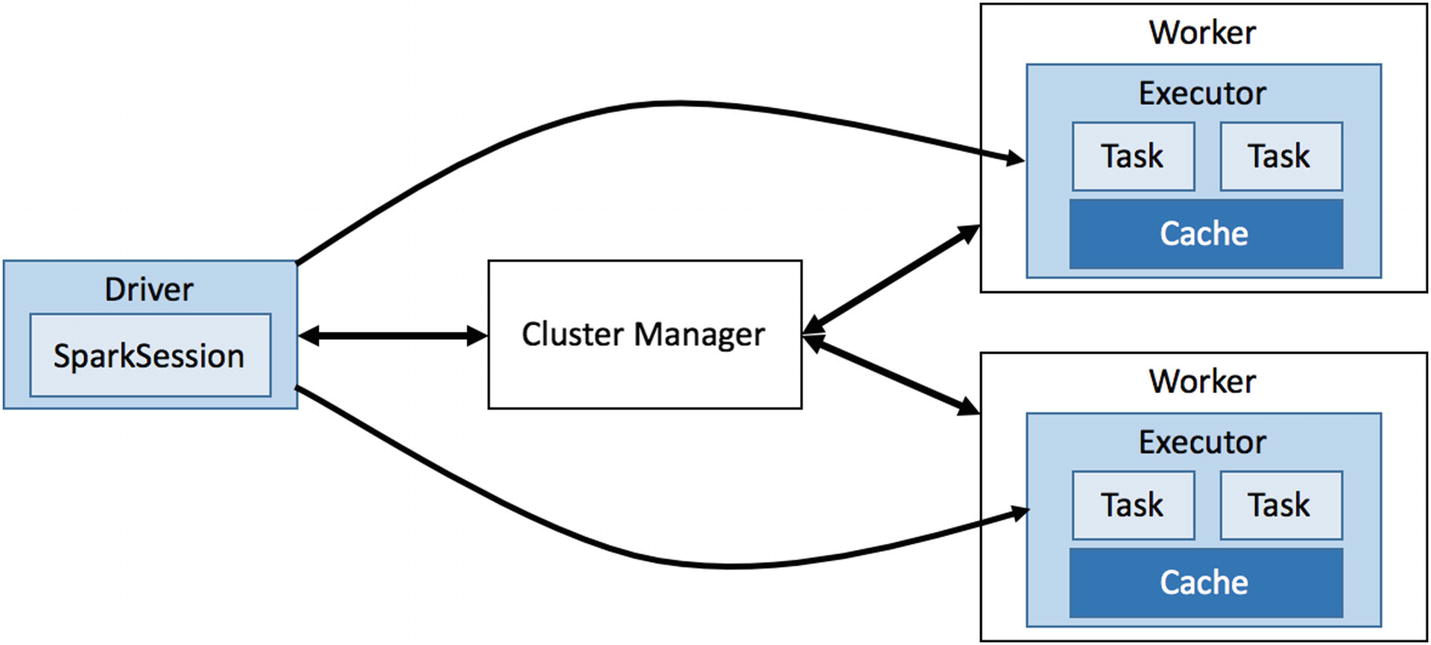
\includegraphics[width=0.7\linewidth]{illustrations/cluster-overview.jpg}
	\caption{ Interaction entre une application Spark et le cluster manager. Source : \cite{eginning-Apache-Spark-2-cluster-overwiew}}
	\label{fig:cluster-overview}
\end{figure}




\subparagraph{ Application Spark}
Une application Spark consiste en deux parties. La première partie concerne la logique décrivant les traitements à appliquer sur les données.  Cette logique est décrite en utilisant les APIs\footnote{API en Java, Scala, Python ou R.} disponibles. La deuxième partie est appelée le \textit{driver}, c'est le coordinateur principal d'une application Spark. Le driver interagit avec le cluster manager afin de trouver les machines sur lesquelles le traitement de données doit être réalisé. Ainsi, pour chacune de ces machines, le driver Spark lance le processus \textit{executor} en passant par le cluster manager. Un autre rôle du  driver Spark est de gérer et de distribuer les tâches Spark en provenance de l'application Spark sur chaque executor. Pour précision , dans la Figure \ref{fig:cluster-overview}, la classe \textit{SparkSession} est le point d'entrée vers une application Spark.

\subparagraph{Spark driver et executor}

Chaque Spark \textit{executor} est alloué exclusivement à une application Spark spécifique et la durée de vie d'un \textit{executor} est celle de l'application Spark. 

Spark utilise l'architecture master-slave. Spark \textit{driver} est le master et Spark \textit{executor} est le slave. De ce fait, une application Spark n'a qu'un seul Spark driver et plusieurs Spark \textit{executors}. Chaque Spark \textit{executor} s'occupe d'un traitement  sur une partie de la totalité des données à analyser. De cette manière,  Spark est capable de traiter  les données de façon parallèle. La Figure \ref{fig:small-cluster-3} illustre un exemple d'un cluster. Ce dernier est composé de trois \textit{executors}.
\begin{figure}[H]
	\centering
	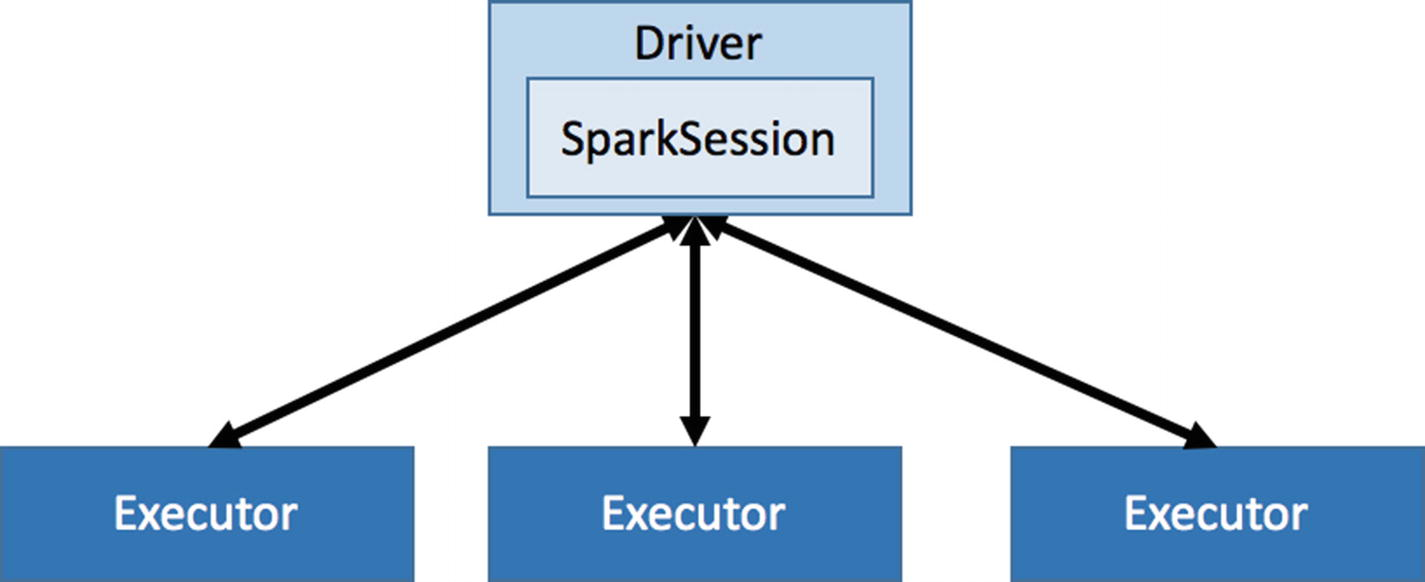
\includegraphics[width=0.7\linewidth]{illustrations/small-cluster-3}
	\caption{Un exemple d'un cluster formé de trois executors. Source : \cite{eginning-Apache-Spark-2-cluster-example}}
	\label{fig:small-cluster-3}
\end{figure}


\subparagraph{Spark Uniffied Stack} Spark offre ce qu'on appelle Spark \textit{Stack}. C'est un ensemble de composantes construites dessus la composante Spark Core.  Ces composantes sont conçues pour répondre à des besoins spécifiques :
\begin{itemize}
	\item Spark SQL  est conçu pour le traitement interactive;
	\item Spark Streaming est utilisé pour les traitements en temps réel;
	\item  GraphX est destiné au traitement de graphe;
	\item MLib est conçu pour  machine learning;
	\item SparkR est consacré au traitement lié au machine learning en utilisant  R.
	
\end{itemize}

\subparagraph{Spark Core} est la base du moteur Spark pour le traitement distribué de données.  On distingue deux parties formant Spark Core. Premièrement, la partie concernant l'infrastructure distribué du calcul. Cette dernière est responsable de la distribution, la coordination et de la planification des tâches  sur les différentes machines formant le cluster. De plus, cette partie gère l'échec d'un traitement donné et le transfert de donnés entre les machines. Le deuxième élément formant Spark Core est appelé RDD (Resilient Distributed Dataset). Un RDD est une collection partitionnée d'objets, tolérante au pannes et en lecture seule. 
La Figure \ref{fig:unified-stack}  présente les différentes entités du Spark Unified Stack avec Spark Core.

\begin{figure}[H]
	\centering
	\captionsetup{justification=centering}
	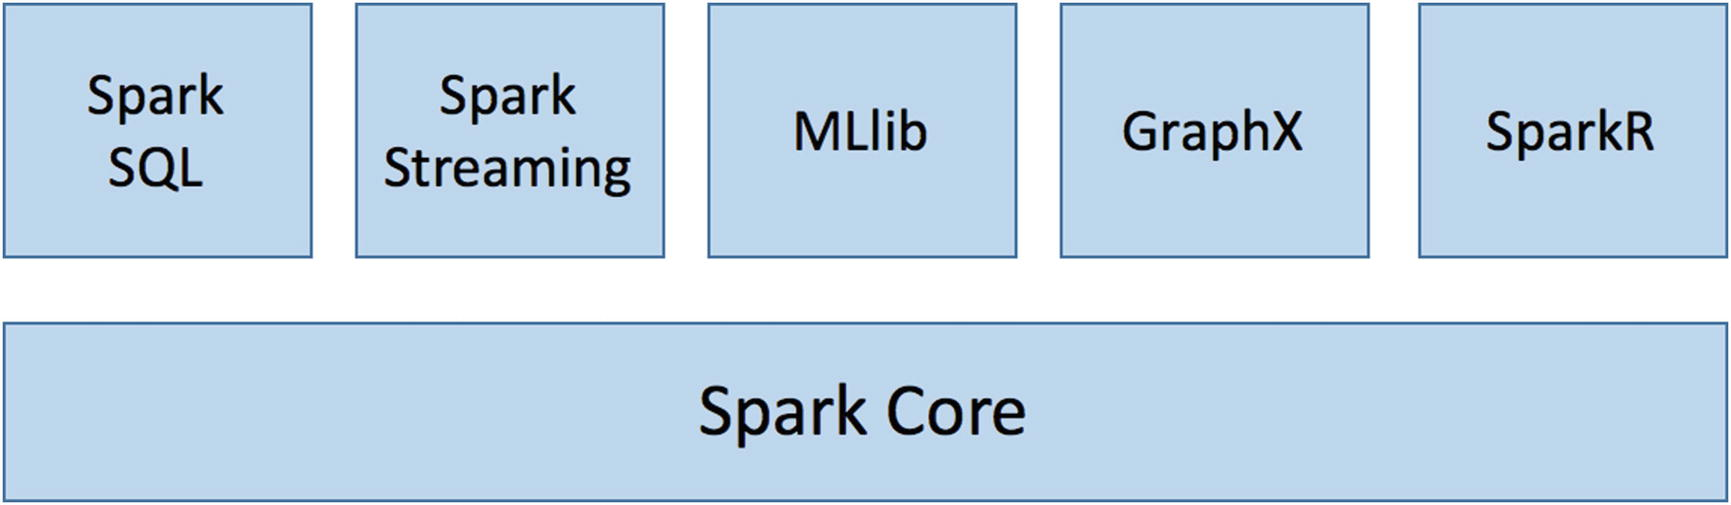
\includegraphics[width=0.7\linewidth]{illustrations/unified-stack}
	\caption{ Spark Unified Stack. Source : \cite{eginning-Apache-Spark-2-unified-stack}}
	\label{fig:unified-stack}
\end{figure}

\paragraph{Resilient Distributed Datasets}~


Spark dispose d'une abstraction notée Resilient Distributed Datasets (ou RDDs). Un RDD est une collection d'objets immuable. Ces objets sont répartis sur les n\oe{}uds du cluster afin d' être traités en parallèle. Un RDD peut être persisté dans la mémoire pour éventuelle réutilisation.   D'ailleurs de cette façon, on constate l'amélioration des performances. En outre, un RDD peut être persisté sur un disque. 

Les RDDs supportent deux types d'opérations sur les objets stockés : les transformations et les actions. Une  transformation appliquée sur un RDD crée un nouveau RDD, par exemple la transformation \textit{filter} retourne un RDD ayant vérifié la condition donnée en entrée.  Toutefois, une action appliquée sur un RDD retourne une seule valeur, par exemple l'action \textit{count} calcule le nombre d'objets d'un RDD. La Figure 	\ref{fig:globalviewrdd} illustre un flux de données avec l'utilisation de Spark. 

\begin{figure}[H]
	\centering
	\captionsetup{justification= centering}
	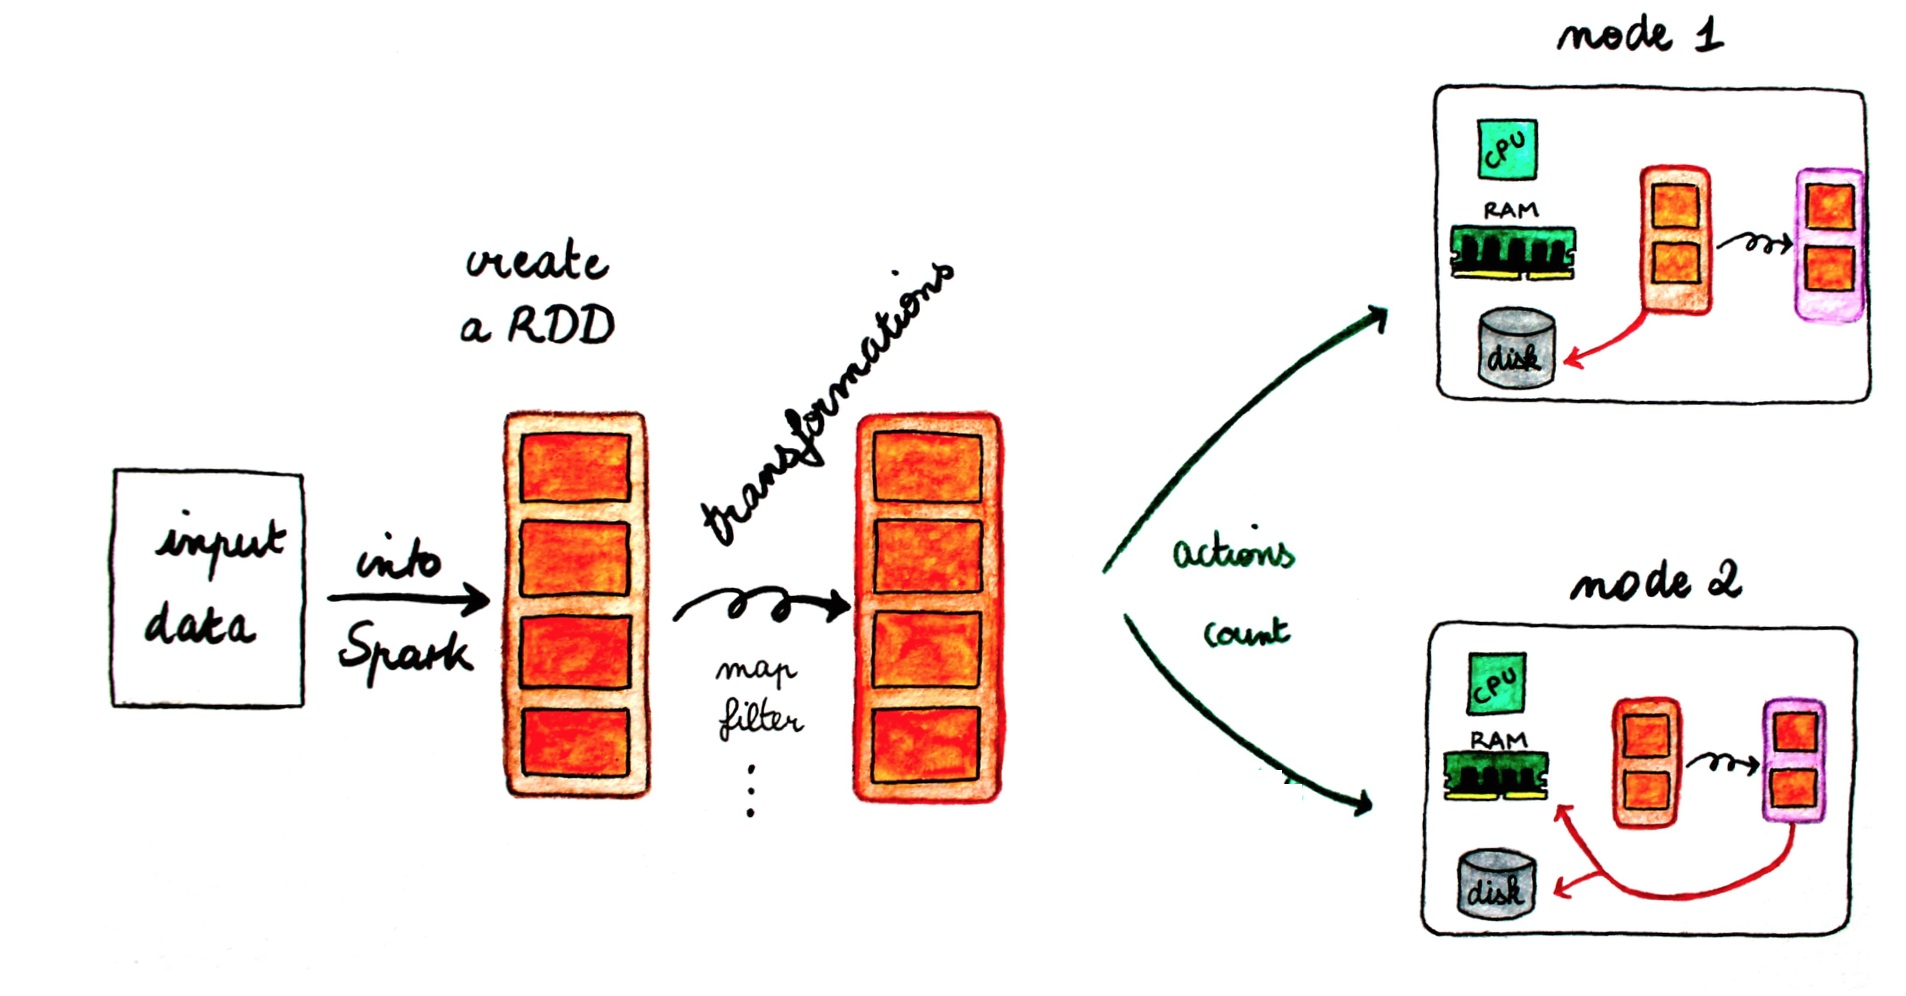
\includegraphics[width=0.7\linewidth]{illustrations/global_view_rdd}
	\caption{Exemple d'un flux de données avec Spark}
	\label{fig:globalviewrdd}
	\source{ \url{https://www.duchess-france.org/starting-with-spark-in-practice/}, consultée le $15/12/2018$.}
\end{figure}

input data sont les données à analyser en utilisant Spark. Ces données sont récupérées depuis des sources extérieures vers Spark. Ce dernier crée un RDD basé sur ces données. Un RDD est représenté par le rectangle en orange, les morceaux en orange dans le rectangle représentent les partitions d'un RDD. 
Il existe plusieurs transformations à appliquer sur un RDD, avec la possibilité d'enchaîner plusieurs transformations. Comme une transformation est à la base  \textit{lazy}, les partitions sont partagées sur les n\oe{}uds du cluster qu'à suite à l'appel d'une action. Une fois une partition est localisé sur un n\oe{}ud donné, les transformations ainsi que les actions peuvent s'enchaîner.

En cas de perte de partition pour une raison ou une autre, Spark est capable de reproduire automatiquement la partition en question. Cette fonctionnalité est assurée via le DAG (Direct Acyclic Graph). Dans ce graphe, Spark enregistre toutes les opérations appliquées sur un RDD.

\section{Conclusion}

Dans ce chapitre,  nous avons décrit brièvement  quelques technologies du Big Data, car la liste de toutes les technologies est très longue. Afin de découvrir ces technologies en pratique, nous allons aborder dans le chapitre \ref{chap:application-on-traceroutes} l'utilisation de ces technologies dans le cas de l'analyse des délais d'un lien décrite dans la chapitre \ref{chap:algorith-detection}.    









